% !TeX program = xelatex
% =====================================================================
%  GRADUATION THESIS (ĐỒ ÁN TỐT NGHIỆP) -- FORM ONLY, NO CONTENT
%  Faculty of Computer Science -- 2026
%
%  Template built from TWO sources:
%  (1) Layout: the sample Capstone Project report (Word) --
%      A4; margins top/bottom 2.0 cm, left 3 cm, right 2 cm
%      (References section: top/bottom 2.5 cm);
%      Times New Roman 13 pt, line spacing 1.3, justified,
%      first-line indent 1.27 cm; chapter heading 18 pt bold centred
%      uppercase; section 14 pt bold; subsection 13 pt bold;
%      sub-subsection 13 pt bold italic; page number centred in footer.
%  (2) Structure & content requirements: "Hướng dẫn nội dung báo cáo
%      Khóa luận tốt nghiệp định hướng Khởi nghiệp & Đổi mới sáng tạo
%      năm 2026" (Phần I -- Khoa KHMT & Khoa KTMT&ĐT):
%        Title page (1 page) -> Contents pages (<=5 pages, numbering
%        style 1.1.1)
%        -> Introduction (unnumbered) (5-7 pages)
%        -> Chapter 1 Literature Review & Background (<=25 pages)
%        -> Chapter 2 Product Design and Development (<=25 pages)
%        -> Chapter 3 Deployment and Business Models (<=5 pages)
%        -> Chapter 4 Conclusion & Recommendations (<=5 pages)
%        -> References, APA style (<=3 pages)
%        -> Appendices (<=10 pages).  TOTAL: <= 100 pages.
%      This is a FORM ONLY: chapter files contain headings and no
%      body content.
%
%  COMPILER: XeLaTeX + Biber (for APA references)
%    Overleaf: Menu > Compiler = XeLaTeX, Main document = main.tex
%              (Overleaf runs Biber automatically.)
%    Local:    xelatex main -> biber main -> xelatex main -> xelatex main
%
%  >>> EDIT ONLY the "THESIS INFORMATION" block below, then write your
%      content in frontmatter/ and chapters/. <<<
% =====================================================================

\documentclass[12pt, a4paper]{report}

% ------------------------- THESIS INFORMATION ------------------------
% Change these values only -- they are used on the title page.
\newcommand{\UniversityName}{VIETNAM KOREA UNIVERSITY OF INFORMATION\\AND COMMUNICATION TECHNOLOGY}
\newcommand{\FacultyName}{Faculty of Computer Science}
\newcommand{\ThesisType}{GRADUATION THESIS}
\newcommand{\ThesisTitle}{Developing an AI-Integrated System to Support the Development of Four Japanese Language Skills – NihonGO}
\newcommand{\StudentOne}{Truong Gia Huy - 22IT119}
\newcommand{\StudentTwo}{Dang Cong Nhat - 22IT204}
\newcommand{\StudentClass}{22JIT}
\newcommand{\Major}{Information Technology}
\newcommand{\Specialization}{Software Engineering}
\newcommand{\Instructor}{Assoc. Prof. PhD. Huynh Cong Phap}
\newcommand{\ThesisCity}{Danang}
\newcommand{\ThesisMonthYear}{December 2026}
% Short lines used in the running header/footer (main part only):
\newcommand{\HeaderTitle}{Developing an AI-Integrated System to Support the Development of Four Japanese Language Skills – NihonGO}
\newcommand{\AuthorLine}{Truong Gia Huy, Dang Cong Nhat - 22JIT}
% ---------------------------------------------------------------------

% ------------------------------ Packages -----------------------------
\usepackage{geometry}
% Margins per QD 675, section 1 (uniform for the whole document):
\geometry{a4paper, top=2cm, bottom=2cm, left=3cm, right=2cm,
          headheight=26pt, footskip=1cm}

\usepackage{fontspec}                 % XeLaTeX fonts
\IfFontExistsTF{Times New Roman}
  {\setmainfont{Times New Roman}}
  {\setmainfont{TeX Gyre Termes}}     % fallback with the same metrics
\usepackage[english]{babel}           % main language: English

\usepackage{setspace}
\usepackage{indentfirst}
\usepackage{titlesec}
\usepackage{tocloft}
\usepackage{fancyhdr}
\usepackage{graphicx}
\graphicspath{{figures/}}
\usepackage{caption}
\usepackage{booktabs}
\usepackage{array}
\usepackage{longtable}
\usepackage{multirow}
\usepackage{amsmath, amssymb}
\usepackage{enumitem}
\usepackage{xcolor}
\usepackage{tikz}                     % cover frame + sample figure
\usetikzlibrary{positioning}


\usepackage{xurl}                    % allow long reference URLs to wrap
\usepackage[hidelinks]{hyperref}      % load hyperref last

% --------------------------- Body typography -------------------------
\AtBeginDocument{\fontsize{13pt}{16.9pt}\selectfont}  % 13 pt, spacing 1.3
\setlength{\parindent}{1.27cm}
\setlength{\parskip}{6pt}
% (body text is justified by default, as in the sample report)

% ------------------------------ Headings -----------------------------
\setcounter{secnumdepth}{3}           % number down to 1.1.1.1
\setcounter{tocdepth}{3}              % TOC down to subsubsection

% Chapter: label and title on ONE line, centred, 18 pt bold uppercase,
% e.g. "CHƯƠNG 1. GIỚI THIỆU" / "PHỤ LỤC A. HƯỚNG DẪN CÀI ĐẶT".
% \@chapapp is "Chương" in the main matter and automatically becomes
% "Phụ lục" after \appendix, so appendix headings print correctly.
\makeatletter
\newcommand{\chapappname}{\@chapapp}
\makeatother
\titleformat{\chapter}[block]
  {\normalfont\fontsize{16pt}{20pt}\selectfont\bfseries\centering}
  {\MakeUppercase{\chapappname} \thechapter.}{0.5em}{\MakeUppercase}
% Chapter headings sit at the very top of the text area: a chapter
% always opens a new page, and Word drops the Heading-1 space-before
% at the top of a page. LaTeX still leaves ~25 pt of line/topskip
% room above a 16 pt heading, so -25 pt compensates for it (measured:
% heading glyphs then start at ~2.2 cm from the paper edge, i.e. at
% the 2 cm top margin, exactly as in the Word sample).
\titlespacing*{\chapter}{0pt}{-25pt}{30pt}

% Section numbering WITH chapter prefix, style 1.1.1 as required by
% the 2026 guidance ("Numbering follows the style 1.1.1, 1.1.2, ...").
\renewcommand{\thesection}{\thechapter.\arabic{section}}
\renewcommand{\thesubsection}{\thesection.\arabic{subsection}}
\renewcommand{\thesubsubsection}{\thesubsection.\arabic{subsubsection}}

% Level 1.1 headings: UPPERCASE, bold, upright (QD 675, section 5).
\titleformat{\section}
  {\normalfont\fontsize{14pt}{18pt}\selectfont\bfseries}
  {\thesection}{0.6em}{\MakeUppercase}
\titlespacing*{\section}{0pt}{12pt}{6pt}

\titleformat{\subsection}
  {\normalfont\fontsize{13pt}{17pt}\selectfont\bfseries}
  {\thesubsection}{0.6em}{}
\titlespacing*{\subsection}{0pt}{10pt}{4pt}

\titleformat{\subsubsection}
  {\normalfont\fontsize{13pt}{17pt}\selectfont\bfseries\itshape}
  {\thesubsubsection}{0.6em}{}
\titlespacing*{\subsubsection}{0pt}{10pt}{4pt}

% Unnumbered chapter (Tóm tắt, Tài liệu tham khảo, ...) styled like a
% chapter heading and added to the Table of Contents.
\newcommand{\unnumberedchapter}[1]{%
  \clearpage
  \phantomsection
  \addcontentsline{toc}{chapter}{#1}%
  \chapter*{\MakeUppercase{#1}}%
}
% Front-matter heading (Nhận xét, Lời cảm ơn): same style, NOT in TOC.
\newcommand{\frontchapter}[1]{%
  \clearpage
  \chapter*{\MakeUppercase{#1}}%
}

% --------------------- Figures, tables, equations --------------------
% Numbered by chapter in the same dotted style: Hình 2.1, Bảng 2.1
\renewcommand{\thefigure}{\thechapter.\arabic{figure}}
\renewcommand{\thetable}{\thechapter.\arabic{table}}
\renewcommand{\theequation}{\thechapter.\arabic{equation}}
% QD 675, section 6: captions in regular (non-bold) type, centred,
% same size as the body text; table caption above, figure caption below.
\captionsetup{justification=centering, labelsep=space, skip=8pt}
\captionsetup[figure]{position=below}   % figure caption BELOW the figure
\captionsetup[table]{position=above}    % table caption ABOVE the table

% ------------------------- Table of contents -------------------------
% Contents/list titles also start exactly at the top margin.
\setlength{\cftbeforetoctitleskip}{-16pt}
\setlength{\cftbeforelottitleskip}{-16pt}
\setlength{\cftbeforeloftitleskip}{-16pt}
\addto\captionsenglish{%
  \renewcommand{\contentsname}{TABLE OF CONTENTS}%
  \renewcommand{\listfigurename}{LIST OF FIGURES}%
  \renewcommand{\listtablename}{LIST OF TABLES}%
  \renewcommand{\figurename}{Figure}%
  \renewcommand{\tablename}{Table}%
}
\renewcommand{\cftchapfont}{\bfseries}
\renewcommand{\cftchappagefont}{\bfseries}
\setlength{\cftbeforechapskip}{6pt}
\renewcommand{\cfttoctitlefont}{\hfill\bfseries\fontsize{16pt}{20pt}\selectfont}
\renewcommand{\cftaftertoctitle}{\hfill}
\renewcommand{\cftloftitlefont}{\hfill\bfseries\fontsize{16pt}{20pt}\selectfont}
\renewcommand{\cftafterloftitle}{\hfill}
\renewcommand{\cftlottitlefont}{\hfill\bfseries\fontsize{16pt}{20pt}\selectfont}
\renewcommand{\cftafterlottitle}{\hfill}

% Save the (numeric) roman page number of the last front-matter page
% so the References can continue the roman sequence on the next pass.
\makeatletter
\providecommand{\FrontLastPage}{5}
\newcommand{\SaveFrontLastPage}{%
  \immediate\write\@auxout{%
    \string\gdef\string\FrontLastPage{\the\value{page}}}}
\makeatother

% Reference list with the QD 675 hanging indent: the label [n] sits
% at the left margin, continuation lines are indented exactly 1 cm.
\newenvironment{refslist}{%
  \setlength{\emergencystretch}{1em}%
  \begin{list}{[\arabic{enumiv}]}{%
    \usecounter{enumiv}%
    \setlength{\leftmargin}{1cm}%
    \setlength{\itemindent}{-1cm}%
    \setlength{\labelwidth}{0.85cm}%
    \setlength{\labelsep}{0.15cm}%
    \setlength{\itemsep}{4pt}%
    \setlength{\parsep}{0pt}}%
}{\end{list}}

% --------------------- Page numbering & header/footer ----------------
% QD 675, sections 1 & 9:
% - Front matter: roman numerals (Acknowledgement i, Contents ii,
%   Abbreviations iii, List of Tables iv, List of Figures v),
%   page number at the bottom right, no header/footer text.
% - Main part (Introduction/Chapter 1 -> Conclusion): arabic numerals;
%   header = thesis title (italic, 11 pt) with a rule below;
%   footer = rule above, author--class (italic, 11 pt) left,
%   page number right.
% - References & Appendices: roman numerals CONTINUING the front
%   sequence (References starts at vi), bottom right, no header text.
\fancypagestyle{front}{%
  \fancyhf{}\fancyfoot[R]{\thepage}%
  \renewcommand{\headrulewidth}{0pt}\renewcommand{\footrulewidth}{0pt}}
\fancypagestyle{mainpart}{%
  \fancyhf{}%
  \fancyhead[L]{\fontsize{11pt}{13pt}\selectfont\itshape \HeaderTitle}%
  \renewcommand{\headrulewidth}{0.4pt}%
  \fancyfoot[L]{\fontsize{11pt}{13pt}\selectfont\itshape \AuthorLine}%
  \fancyfoot[R]{\fontsize{11pt}{13pt}\selectfont\itshape \thepage}%
  \renewcommand{\footrulewidth}{0.4pt}}
\pagestyle{front}
\fancypagestyle{plain}{%
  \fancyhf{}\fancyfoot[R]{\thepage}%
  \renewcommand{\headrulewidth}{0pt}\renewcommand{\footrulewidth}{0pt}}

% =====================================================================
\begin{document}

% ------------------------- Front matter ------------------------------
% Order and roman numbering exactly as the sample Contents page of
% QD 675: Acknowledgement i, Contents ii, Abbreviations iii,
% List of Tables iv, List of Figures v.
\pagenumbering{roman}

% =====================================================================
%  COVERS -- main cover (trang bia chinh) + inner cover (trang phu bia),
%  identical, following "Mau 3" of QD 675:
%    University name (regular) / Faculty (bold, 16 pt) / VKU logo /
%    GRADUATION THESIS (bold, 25 pt) / thesis title (uppercase, bold, 16 pt) /
%    student block (bold labels, 14 pt) / Danang - month/year (bold).
%  Single-line frame. All text comes from main.tex (THESIS INFORMATION).
% =====================================================================
\newcommand{\makecoverpage}{%
  \begin{titlepage}
  \thispagestyle{empty}
  \begin{tikzpicture}[remember picture, overlay]
    \draw[line width=0.8pt]
      ([xshift=2.2cm, yshift=-2.2cm]current page.north west)
      rectangle
      ([xshift=-2.2cm, yshift=2.2cm]current page.south east);
  \end{tikzpicture}

  \begin{center}
    {\fontsize{16pt}{20pt}\selectfont \UniversityName \par}
    \vspace{6pt}
    {\fontsize{16pt}{20pt}\selectfont\bfseries \FacultyName \par}

    \vspace{1.0cm}
    % VKU logo, centred between the faculty name and the thesis type
    % (position as in Mau 3 of QD 675). File: figures/logo.png
    
\includegraphics[width=4.5cm]{logo.png}\par
    \vspace{0.6cm}

    {\fontsize{25pt}{30pt}\selectfont\bfseries \ThesisType \par}

    \vspace{1.2cm}
    \begin{minipage}{0.88\textwidth}
      \centering
      \fontsize{16pt}{22pt}\selectfont\bfseries
      \MakeUppercase{\ThesisTitle}\par
    \end{minipage}\par

    \vspace{2.2cm}
    \begin{minipage}{0.85\textwidth}
      \fontsize{14pt}{20pt}\selectfont
      \begin{tabular}{@{}l@{\hspace{0.4cm}}l@{}}
        \textbf{Student:}       & \StudentOne \\
                                 & \StudentTwo \\
        \textbf{Class:}          & \StudentClass \\
        \textbf{Major:}          & \Major \\
        \textbf{Specialization:} & \Specialization \\
        \textbf{Supervisor:}     & \Instructor \\
      \end{tabular}
    \end{minipage}

    \vfill
    {\fontsize{14pt}{18pt}\selectfont\bfseries
      \ThesisCity{} - \ThesisMonthYear \par}
    \vspace{1cm}
  \end{center}
  \end{titlepage}
}

\makecoverpage   % main cover (trang bia chinh)
\makecoverpage   % inner cover (trang phu bia)
            % main cover + inner cover
\setcounter{page}{1}                  % covers are not counted -> Ack. = i
% =====================================================================
%  ACKNOWLEDGEMENT
% =====================================================================
\phantomsection
\addcontentsline{toc}{chapter}{ACKNOWLEDGEMENT}
\frontchapter{Acknowledgement}

Throughout the completion of our graduation thesis on NihonGO, a system designed to support Japanese language learning, we have received guidance, support, and encouragement from our lecturers, families, and friends. We would like to express our sincere gratitude to everyone who has supported us throughout our studies and the development of this project.

First, we would like to thank the lecturers of the Faculty of Computer Science at the Vietnam--Korea University of Information and Communication Technology, the University of Danang. The knowledge and working methods we acquired during our studies provided the foundation for analysing, designing, and developing the system presented in this thesis.

In particular, we are deeply grateful to our supervisor, Assoc. Prof. PhD. Huynh Cong Phap. His guidance and constructive feedback helped us define the direction of our project, gain a clearer understanding of the problems to be addressed, and progressively improve both this thesis and the NihonGO system.

We also thank everyone who took the time to participate in our survey and share their experiences of learning Japanese. Their accounts of difficulties, expectations, and suggestions helped us better understand learners' needs and informed our decisions on the system's features and development direction.

We would also like to thank our families and friends for their continued care, encouragement, and support throughout our studies. Their presence and support motivated us to persevere and complete this graduation thesis.

Given our limited experience and the time available, this work may still contain shortcomings. We welcome feedback from our lecturers and fellow students to help us deepen our knowledge and further improve the thesis and the system.

To all who have supported us, we offer our sincere thanks.

\vspace{1.5cm}
\begin{flushright}
  \begin{minipage}{0.5\textwidth}
    \centering
    The Authors\\[1.2cm]
    \textbf{\StudentOne}\\[2pt]
    \textbf{\StudentTwo}
  \end{minipage}
\end{flushright}
  % i

\clearpage
\phantomsection
\addcontentsline{toc}{chapter}{TABLE OF CONTENTS}
\tableofcontents                     % ii

% =====================================================================
%  LIST OF ABBREVIATIONS (optional, QD 675 sec. 3.1): alphabetical
%  table placed in the front matter. Delete the \input line in
%  main.tex if the thesis uses no abbreviations.
% =====================================================================
\clearpage
\phantomsection
\addcontentsline{toc}{chapter}{LIST OF ABBREVIATIONS}
\chapter*{LIST OF ABBREVIATIONS}

\begin{center}
\begin{tabular}{@{}p{3cm}p{11.5cm}@{}}
  \textbf{API} & Application Programming Interface \\
  \textbf{AWS} & Amazon Web Services \\
  \textbf{EC2} & Amazon Elastic Compute Cloud \\
  \textbf{LLM} & Large Language Model \\
  \textbf{NLP} & Natural Language Processing \\
  % Add your abbreviations here, in alphabetical order...
\end{tabular}
\end{center}
    % iii (optional)

\clearpage
\phantomsection
\addcontentsline{toc}{chapter}{LIST OF TABLES}
\listoftables                        % iv

\clearpage
\phantomsection
\addcontentsline{toc}{chapter}{LIST OF FIGURES}
\listoffigures                       % v
\SaveFrontLastPage

% --------------------------- Main matter -----------------------------
% Arabic numbering from page 1, with header/footer (QD 675, sec. 9).
\clearpage
\pagenumbering{arabic}
\pagestyle{mainpart}
\fancypagestyle{plain}{%
  \fancyhf{}%
  \fancyhead[L]{\fontsize{11pt}{13pt}\selectfont\itshape \HeaderTitle}%
  \renewcommand{\headrulewidth}{0.4pt}%
  \fancyfoot[L]{\fontsize{11pt}{13pt}\selectfont\itshape \AuthorLine}%
  \fancyfoot[R]{\fontsize{11pt}{13pt}\selectfont\itshape \thepage}%
  \renewcommand{\footrulewidth}{0.4pt}}

% Introduction has no chapter/section numbers; its tables use plain numbers.
\begingroup
\setcounter{secnumdepth}{0}
\renewcommand{\thetable}{\arabic{table}}
% Nội dung tiếng Việt; tiêu đề giữ tiếng Anh.
% Số liệu tổng hợp từ 48 phản hồi khảo sát do nhóm cung cấp.
\unnumberedchapter{INTRODUCTION}
\label{chap:introduction}

\section{MOTIVATION}

Một người học có thể nhớ nghĩa của một từ tiếng Nhật nhưng vẫn lúng túng khi dùng từ đó để trả lời một câu hỏi. Họ có thể hiểu mẫu ngữ pháp trong sách, nhưng khi nghe một đoạn hội thoại lại không nhận ra mẫu câu vừa học. Khoảng cách giữa việc ghi nhớ kiến thức và sử dụng được ngôn ngữ là vấn đề mà đề tài NihonGO hướng đến. Để thu hẹp khoảng cách này, người học cần có cơ hội luyện tập, được giải thích những phần chưa hiểu và thường xuyên vận dụng lại kiến thức đã học.

Trong bối cảnh chuyển đổi số trong giáo dục, việc tự học có thể diễn ra qua ứng dụng di động, video, từ điển trực tuyến và các công cụ AI. Những hình thức này giúp người học chủ động lựa chọn thời gian và nội dung phù hợp với bản thân. Tuy nhiên, có nhiều tài liệu và công cụ để lựa chọn cũng đặt ra một câu hỏi thực tế: người học nên bắt đầu từ đâu, ôn lại như thế nào và làm sao biết mình đang tiến bộ? Với sinh viên phải sắp xếp việc học ngoại ngữ cùng các môn chuyên ngành, sự thuận tiện và rõ ràng trong quá trình học có ý nghĩa thiết thực.

Tiếng Nhật còn đặt ra yêu cầu kết hợp nhiều loại kiến thức. Bên cạnh Hiragana và Katakana, người học cần ghi nhớ Kanji, cách đọc, từ vựng và các mẫu ngữ pháp. Những kiến thức này tiếp tục xuất hiện trong cả bốn kỹ năng nghe, nói, đọc và viết. Vì vậy, một hệ thống hỗ trợ học tiếng Nhật cần giúp người học thấy được mối liên hệ giữa điều vừa học và cách sử dụng trong ngữ cảnh cụ thể. Đây là hướng tiếp cận được nhóm lựa chọn khi xây dựng NihonGO.

\subsection{Learner Needs from the Survey}

Để tìm hiểu những khó khăn thực tế, nhóm sử dụng dữ liệu khảo sát gồm 48 phản hồi được ghi nhận từ ngày 16/09/2026 đến ngày 17/11/2026. Nội dung khảo sát xoay quanh trình độ hiện tại, khó khăn khi học tiếng Nhật, công cụ đang sử dụng và những chức năng người học mong muốn. Trong số người tham gia, 47 người là sinh viên và một người học vì sở thích. Về trình độ tự đánh giá, 37 người ở mức N5--N4, hai người vừa bắt đầu, sáu người ở mức N3 và ba người ở mức N2--N1. Nhóm mới bắt đầu và N5--N4 chiếm 81,3\%, cho thấy nhu cầu của người học ở giai đoạn xây dựng nền tảng là trọng tâm đáng quan tâm trong mẫu khảo sát.

\begin{table}[htbp]
  \centering
  \caption{Các khó khăn đối với người bắt đầu học tiếng Nhật được lựa chọn trong khảo sát}
  \label{tab:initial-learning-difficulties}
  \begin{tabular}{@{}p{10cm}rr@{}}
    \toprule
    \textbf{Khó khăn} & \textbf{Số người} & \textbf{Tỷ lệ} \\
    \midrule
    Ghi nhớ nét viết và ý nghĩa Kanji & 36 & 75,0\% \\
    Duy trì động lực và tần suất học tập & 35 & 72,9\% \\
    Xây dựng vốn từ vựng nền tảng & 20 & 41,7\% \\
    Phát âm chính xác và trọng âm & 13 & 27,1\% \\
    Học và ghi nhớ Hiragana, Katakana & 10 & 20,8\% \\
    \bottomrule
  \end{tabular}
  \par\smallskip
  {\fontsize{11pt}{14pt}\selectfont Nguồn: tổng hợp từ 48 phản hồi khảo sát của đề tài. Câu hỏi cho phép chọn nhiều đáp án; tỷ lệ được tính trên 48 người trả lời.\par}
\end{table}

Bảng~\ref{tab:initial-learning-difficulties} trình bày ý kiến của toàn bộ người tham gia về khó khăn đối với người bắt đầu học. Kanji và việc duy trì động lực là hai nội dung được lựa chọn nhiều nhất. Điều này gợi ý rằng sản phẩm cần quan tâm đồng thời đến cách học và trải nghiệm học. Người học cần được hỗ trợ ghi nhớ kiến thức, nhưng cũng cần có lý do để quay lại luyện tập mỗi ngày và nhận thấy kết quả từ những lần luyện tập đó.

Các câu trả lời mở giúp làm rõ hơn những con số trên. Có người mong muốn học Kanji qua bộ thủ và câu chuyện để dễ liên tưởng; có người muốn lưu kiến thức đã học vào một nơi thuận tiện để tìm lại. Một số ý kiến đề nghị bổ sung ví dụ từ video, bài hát hoặc những câu nói quen thuộc để việc học từ vựng bớt đơn điệu. Những mong muốn này cho thấy người học quan tâm đến cách kiến thức được giải thích, ghi nhớ và ôn lại, bên cạnh số lượng bài học được cung cấp.

Một vấn đề khác là thiếu cơ hội giao tiếp. Trong khảo sát, có người cho biết đã học từ vựng và ngữ pháp nhưng khi nói vẫn chưa tạo được một câu hoàn chỉnh. Những người khác muốn trò chuyện với AI, nghe lại bản thu hoặc được góp ý về cách dùng từ. Có phản hồi nêu khó khăn khi tự luyện phát âm qua video: người học nghe và bắt chước nhưng không biết mình sai ở đâu. Các ý kiến này là cơ sở để nhóm chú trọng hoạt động thực hành và phản hồi trong thiết kế sản phẩm.

Khảo sát cũng ghi nhận việc sử dụng nhiều công cụ: 36 người chọn Mazii, 30 người chọn Quizlet, 19 người chọn Anki và 45 người chọn ChatGPT, Gemini hoặc công cụ trò chuyện AI khác. Người trả lời được chọn nhiều phương án, nên một người có thể sử dụng đồng thời nhiều công cụ. Một số phản hồi đánh giá các ứng dụng hiện có hữu ích cho tra cứu và ghi nhớ; một số khác vẫn mong muốn được hỗ trợ thêm về giao tiếp, lộ trình và ôn tập. Các ý kiến về chi phí cũng gợi mở yêu cầu cân nhắc khả năng tiếp cận của sinh viên khi đề xuất mô hình kinh doanh.

Với quy mô 48 phản hồi và thành phần chủ yếu là sinh viên, khảo sát được dùng để định hướng sản phẩm cho nhóm người dùng ban đầu. Trình độ trong khảo sát là thông tin người học tự đánh giá. Những kết quả này chưa đại diện cho toàn bộ thị trường học tiếng Nhật, nhưng cung cấp các vấn đề cụ thể để nhóm lựa chọn và giải quyết trong phạm vi đồ án.

\subsection{The Direction of NihonGO}

Từ những nhu cầu trên, NihonGO được định hướng trở thành một môi trường học tập kết hợp kiến thức nền tảng với thực hành bốn kỹ năng. Chẳng hạn, khi gặp một từ mới trong bài đọc, người học cần hiểu nghĩa và cách dùng của từ; sau đó có thể ôn lại bằng flashcard và thử vận dụng trong bài viết hoặc hội thoại. Sự kết nối này là mục tiêu thiết kế của hệ thống, giúp mỗi hoạt động học có ý nghĩa rõ ràng trong quá trình sử dụng tiếng Nhật.

AI được lựa chọn để hỗ trợ những hoạt động cần tương tác, như trò chuyện theo tình huống, giải thích một phần nội dung bài đọc hoặc góp ý bài viết. Các thành phần nhận dạng và tổng hợp tiếng nói hỗ trợ chuyển đổi giữa âm thanh và văn bản, tạo điều kiện xây dựng hoạt động luyện nói và nghe lại. Ví dụ, với một tình huống gọi món, người học có thể thử lựa chọn cách diễn đạt, tiếp nhận câu trả lời và tiếp tục cuộc hội thoại. Cách tổ chức này hướng đến việc tạo thêm cơ hội luyện tập ngoài lớp học.

Bên cạnh các chức năng AI, hệ thống cần có học liệu, công cụ tra cứu và cách lưu kết quả rõ ràng. Đây là những thành phần giúp người học tiếp tục ôn tập sau một lần tương tác. Từ định hướng đó, nhóm lựa chọn đề tài \textit{Developing an AI-Integrated System to Support the Development of Four Japanese Language Skills -- NihonGO}. Đề tài tập trung xây dựng một sản phẩm có thể dùng thử, đánh giá và tiếp tục hoàn thiện từ trải nghiệm thực tế của người học.

\section{OBJECTIVES AND CONTRIBUTIONS}

\subsection{General Objective}

Mục tiêu tổng quát của đề tài là xây dựng NihonGO, hệ thống tích hợp AI hỗ trợ phát triển bốn kỹ năng nghe, nói, đọc và viết tiếng Nhật. Hệ thống hướng đến người học tiếng Nhật ở mọi trình độ, có nhu cầu tự học hoặc luyện tập bổ sung bên cạnh các khóa học. Thông qua việc kết hợp bài luyện, tra cứu, ôn tập và phản hồi, NihonGO tạo điều kiện để người học củng cố kiến thức và thử vận dụng vào những tình huống cụ thể.

Trong phạm vi đồ án, nhóm hướng đến một phiên bản sản phẩm khả dụng tối thiểu (Minimum Viable Product -- MVP). Đây là phiên bản có các chức năng cốt lõi đủ để người học trải nghiệm quá trình học và để nhóm kiểm tra mức độ phù hợp của giải pháp. Kết quả dùng thử sẽ làm cơ sở hoàn thiện sản phẩm, lựa chọn chức năng ưu tiên và đề xuất hướng phát triển thương mại sau đồ án.

\subsection{Specific Objectives}

Các mục tiêu cụ thể được xác định theo quá trình xây dựng sản phẩm:

\begin{enumerate}[leftmargin=*, itemsep=4pt]
  \item \textbf{Phân tích nhu cầu người học.} Tổng hợp dữ liệu khảo sát, xác định những khó khăn nổi bật và chuyển thành yêu cầu của hệ thống. Kết quả cần làm rõ sản phẩm phục vụ ai, hỗ trợ hoạt động nào và chức năng nào cần được ưu tiên.
  \item \textbf{Thiết kế hệ thống.} Xây dựng kiến trúc, cơ sở dữ liệu và giao diện cho các hoạt động học tập. Thiết kế cần giúp người dùng dễ tìm bài luyện, thực hiện nhiệm vụ và xem lại kết quả; đồng thời thuận tiện cho việc bảo trì, bổ sung học liệu và mở rộng chức năng.
  \item \textbf{Xây dựng phiên bản MVP.} Phát triển các chức năng luyện nghe, hội thoại theo tình huống, đọc hiểu và luyện viết; kết hợp tra cứu từ vựng, Kanji, flashcard và theo dõi học tập. Mỗi chức năng cần có một quá trình sử dụng rõ ràng từ khi bắt đầu đến khi nhận kết quả.
  \item \textbf{Tích hợp AI vào hoạt động học.} Sử dụng AI để hỗ trợ hội thoại, giải thích và góp ý theo nội dung người học đang luyện tập. Phản hồi cần dễ hiểu, liên quan đến bài học và được trình bày sao cho người học biết phần nào cần xem lại hoặc tiếp tục thực hành.
  \item \textbf{Kiểm thử và đánh giá sản phẩm.} Kiểm tra độ ổn định của các chức năng, khả năng lưu dữ liệu, thời gian phản hồi và cách xử lý lỗi. Kết hợp dùng thử để tìm hiểu người học có hoàn thành được hoạt động chính hay không và còn gặp trở ngại ở bước nào.
  \item \textbf{Đề xuất mô hình kinh doanh.} Xác định giá trị của NihonGO đối với người dùng, nhóm khách hàng ban đầu và phương án duy trì sản phẩm. Việc đề xuất gói sử dụng cần cân nhắc cả chi phí vận hành AI lẫn khả năng chi trả của sinh viên.
\end{enumerate}

\subsection{Expected Contributions}

Kết quả dự kiến của đề tài gồm bản phân tích nhu cầu, thiết kế hệ thống và phiên bản NihonGO có thể triển khai dùng thử. Điểm đóng góp của sản phẩm nằm ở cách tổ chức các hoạt động học tiếng Nhật có liên hệ với nhau: từ tiếp cận kiến thức, luyện tập đến xem lại và ôn tập. Các nhu cầu được nêu trong khảo sát, như khó ghi nhớ Kanji, thiếu cơ hội nói và khó duy trì việc học, là cơ sở để giải thích các lựa chọn chức năng.

Về kỹ thuật, đề tài vận dụng các công nghệ sẵn có để xây dựng một hệ thống học tập hoàn chỉnh ở quy mô MVP. Nhóm tập trung vào cách kết hợp ứng dụng, dữ liệu học tập và dịch vụ AI để phục vụ nhiệm vụ cụ thể của người học. Quá trình kiểm thử và dùng thử giúp ghi nhận những điểm làm được, những hạn chế còn tồn tại và các phần cần ưu tiên khi phát triển phiên bản tiếp theo.

\section{SCOPE OF THE THESIS}

\subsection{Target Users}

NihonGO hướng đến người học tiếng Nhật ở tất cả các trình độ, từ người mới bắt đầu đến người học ở các mức N5, N4, N3, N2 và N1. Đối tượng sử dụng bao gồm sinh viên, người đi làm và người tự học vì sở thích hoặc mục tiêu cá nhân. Tùy theo trình độ và nhu cầu, người học có thể lựa chọn nội dung để xây dựng kiến thức nền tảng, củng cố kỹ năng hoặc luyện cách sử dụng tiếng Nhật trong những ngữ cảnh phức tạp hơn.

Hệ thống hỗ trợ cả việc tự học độc lập và luyện tập bổ sung bên cạnh các khóa học. Người mới bắt đầu có thể làm quen với chữ viết, từ vựng và mẫu câu cơ bản; người đã có nền tảng có thể luyện nghe, hội thoại, đọc hiểu và diễn đạt bằng văn bản theo trình độ của mình. Dù mẫu khảo sát chủ yếu là sinh viên ở mức N5--N4, đối tượng phục vụ của NihonGO được xác định rộng hơn, nhằm đáp ứng nhu cầu học tập xuyên suốt từ cơ bản đến nâng cao.

\subsection{Functional and Technology Scope}

Phạm vi chức năng của hệ thống được tổ chức theo bốn kỹ năng, với các công cụ kiến thức nền tảng dùng chung:

\begin{itemize}[leftmargin=*, itemsep=4pt]
  \item \textbf{Nghe:} luyện nghe với nội dung âm thanh hoặc video có văn bản hỗ trợ; cho phép theo dõi nội dung và thực hành nghe, nhắc lại theo từng phần.
  \item \textbf{Nói:} luyện hội thoại với AI theo tình huống, sử dụng kiến thức đã học để tạo câu trả lời và xem lại nội dung tương tác.
  \item \textbf{Đọc:} đọc văn bản, trả lời câu hỏi và xem giải thích gắn với nội dung bài; hỗ trợ tìm hiểu từ vựng và cấu trúc câu khi gặp phần chưa hiểu.
  \item \textbf{Viết:} luyện diễn đạt bằng văn bản, lưu bản nháp hoặc bài nộp và tiếp nhận góp ý để xem xét chỉnh sửa.
  \item \textbf{Tra cứu và ôn tập:} cung cấp công cụ tra từ, tìm hiểu Kanji và học bằng flashcard; lưu thông tin học tập để người dùng thuận tiện tiếp tục ở những lần sau.
\end{itemize}

Về công nghệ, ứng dụng sử dụng React Native và TypeScript; dịch vụ máy chủ được xây dựng bằng Flask và dữ liệu học tập được quản lý bằng PostgreSQL. Phiên bản web cho phép truy cập bằng trình duyệt. AI và các thành phần xử lý tiếng nói được tích hợp theo yêu cầu của từng chức năng. Cách lựa chọn và kết nối các thành phần này được trình bày chi tiết ở Chương 2.

\subsection{System Limitations}

Trong phạm vi đồ án, nhóm ưu tiên hoàn thiện các hoạt động học cốt lõi trên bộ học liệu được chuẩn bị. Nội dung và mức độ hỗ trợ có thể khác nhau giữa các trình độ. Những mong muốn mở rộng từ khảo sát, như kết nối trực tiếp với người bản xứ, gọi video hoặc xây dựng lộ trình tự động cho từng cá nhân, được xem xét cho các giai đoạn phát triển sau.

Phản hồi của AI được dùng để hỗ trợ người học và có thể có sai sót. Đặc biệt, việc chuyển giọng nói thành văn bản chưa đủ để kết luận người học phát âm đúng hoặc sai ở từng âm, nên khả năng chấm phát âm cần được đánh giá riêng. Các hoạt động phụ thuộc AI và dữ liệu trên máy chủ cần kết nối Internet. Hệ thống không thay thế vai trò hướng dẫn của giáo viên và không cung cấp chứng nhận năng lực tiếng Nhật.

Đánh giá trong đồ án tập trung vào chức năng, độ ổn định và trải nghiệm dùng thử. Việc xác định người học tiến bộ bao nhiêu sau một thời gian sử dụng cần có quá trình theo dõi và kiểm tra đầu vào, đầu ra phù hợp. Vì vậy, kết quả khảo sát nhu cầu ban đầu được dùng để định hướng thiết kế, không được xem là bằng chứng về hiệu quả học tập của sản phẩm.

\subsection{Deployment Environment}

Hệ thống được phát triển và kiểm thử trên máy cục bộ trước khi đưa lên môi trường dùng thử qua Internet. Người dùng truy cập bằng ứng dụng hoặc trình duyệt; các hoạt động hội thoại bằng giọng nói cần thiết bị có micro và quyền ghi âm. Máy chủ tiếp nhận yêu cầu, xử lý dữ liệu học tập và kết nối đến các dịch vụ AI cần thiết.

Môi trường triển khai cần hỗ trợ quản lý tài khoản, bảo vệ dữ liệu và lưu kết quả theo đúng người dùng. Khóa truy cập dịch vụ AI được quản lý ở phía máy chủ. Trong quá trình dùng thử, nhóm sẽ theo dõi lỗi, thời gian phản hồi và chi phí để điều chỉnh cấu hình phù hợp với quy mô sử dụng. Đây cũng là cơ sở để xem xét khả năng mở rộng khi sản phẩm có thêm người học.

\section{RESEARCH METHODS}

Đề tài được thực hiện theo quá trình khảo sát, thiết kế, xây dựng và đánh giá. Trước hết, nhóm tổng hợp câu trả lời để xác định người dùng đang gặp khó khăn gì và mong muốn được hỗ trợ như thế nào. Các câu hỏi lựa chọn được thống kê theo số người và tỷ lệ; câu trả lời mở được đọc và nhóm theo những nội dung gần nhau, như ghi nhớ kiến thức, giao tiếp, động lực và chi phí. Thông tin liên hệ của người trả lời không được đưa vào báo cáo.

Từ kết quả phân tích, nhóm xác định yêu cầu và thiết kế các hoạt động học tương ứng. Chẳng hạn, nhu cầu luyện giao tiếp được cụ thể hóa thành chức năng hội thoại theo tình huống; nhu cầu ghi nhớ và tìm lại kiến thức được thể hiện qua tra cứu, flashcard và dữ liệu học tập. Việc phát triển được chia thành từng phần để có thể kiểm tra sớm, nhận diện vướng mắc và điều chỉnh trước khi bổ sung chức năng tiếp theo.

Sau khi xây dựng, nhóm kiểm thử các hoạt động chính như đăng nhập, chọn bài, thực hiện bài luyện và xem lại kết quả. Với chức năng AI, việc đánh giá chú ý đến sự phù hợp của câu trả lời, mức độ dễ hiểu và thời gian chờ. Phản hồi dùng thử giúp xác định những bước còn khó sử dụng và nội dung cần cải thiện. Các kết quả được trình bày cùng điều kiện kiểm tra trong Chương 3 để làm rõ mức độ đáp ứng của sản phẩm.

\section{SCIENTIFIC AND PRACTICAL SIGNIFICANCE}

Ý nghĩa thực tiễn của NihonGO bắt đầu từ những hoạt động gần với nhu cầu tự học: có nơi tra lại từ vừa gặp, có bài để luyện, có cơ hội thử nói và có phản hồi để xem lại cách diễn đạt. Khi được tổ chức thuận tiện trong một hệ thống, những hoạt động này có thể giúp người học chủ động hơn trong việc ôn kiến thức và bố trí thời gian luyện tập. Đối với sinh viên, đây là hướng hỗ trợ bổ sung cho việc học trên lớp và những thời điểm chưa có người cùng thực hành.

Đề tài cũng tạo cơ hội vận dụng kiến thức về phát triển phần mềm và AI vào một bài toán cụ thể. Thay vì chỉ dừng ở việc kết nối một dịch vụ AI, nhóm cần giải quyết cách chuẩn bị nội dung, lưu dữ liệu, trình bày phản hồi và tổ chức quá trình học. Những kinh nghiệm từ quá trình xây dựng, kiểm thử và dùng thử có thể tiếp tục được sử dụng để cải thiện sản phẩm hoặc nghiên cứu cách hỗ trợ học ngoại ngữ bằng công nghệ.

Về định hướng khởi nghiệp, NihonGO có thể bắt đầu từ nhóm sinh viên có nhu cầu tự học, sau đó xem xét mở rộng học liệu và hợp tác với câu lạc bộ hoặc đơn vị đào tạo. Một phương án kinh doanh cần nghiên cứu là duy trì các chức năng cơ bản miễn phí và cung cấp gói nâng cao cho những hoạt động có chi phí AI lớn hơn. Trước khi lựa chọn mức giá và mở rộng, nhóm cần tiếp tục tìm hiểu người dùng có quay lại học thường xuyên hay không, chức năng nào được sử dụng nhiều và giá trị nào khiến họ sẵn sàng trả phí. Đây là các bước cần thiết để phát triển từ một đồ án kỹ thuật thành sản phẩm có khả năng duy trì lâu dài.

\section{THESIS STRUCTURE}

Báo cáo gồm phần Introduction và bốn chương. Phần Introduction giới thiệu lý do chọn đề tài, nhu cầu người học, mục tiêu và phạm vi thực hiện. Chương 1 trình bày cơ sở lý thuyết, tìm hiểu các sản phẩm liên quan và xác định yêu cầu hệ thống. Chương 2 mô tả kiến trúc, cơ sở dữ liệu, giao diện và cách xây dựng các chức năng của NihonGO. Chương 3 trình bày kết quả triển khai, kiểm thử, đánh giá và đề xuất mô hình kinh doanh. Chương 4 tổng hợp kết quả đạt được, các hạn chế và hướng phát triển tiếp theo.
   % Unnumbered Introduction
\clearpage
\endgroup
\setcounter{secnumdepth}{3}
% Nội dung 2.1--2.3: tiếng Việt, tiêu đề tiếng Anh.
\chapter{Literature Review and Background}
\label{chap:background}

\section{FIELD OVERVIEW}

\subsection{Technology Trends and Digital Transformation}

Một buổi tự học tiếng Nhật có thể gồm nhiều hoạt động: đọc bài, tra từ mới, nghe cách phát âm, làm bài tập và ôn lại kiến thức. Khi sử dụng các công cụ riêng cho từng việc, người học phải tự chuyển nội dung giữa chúng. Chẳng hạn, sau khi tra một từ trong bài đọc, họ cần ghi lại từ đó rồi tạo thẻ để ôn vào ngày hôm sau. Vấn đề đặt ra cho NihonGO là làm cho những bước này thuận tiện hơn và giúp người học tiếp tục sử dụng kiến thức vừa học.

Các công cụ học tập số cung cấp những cách hỗ trợ khác nhau. Từ điển giúp tìm nghĩa và cách dùng của từ. Flashcard, hay thẻ ghi nhớ, hỗ trợ ôn tập. Công cụ hội thoại tạo cơ hội thực hành nghe và trả lời. Trong đề tài này, nhóm xem xét ba hướng công nghệ liên quan trực tiếp đến những hoạt động đó.

\textbf{Thứ nhất, lưu kết quả để tổ chức ôn tập.} Với thẻ ghi nhớ điện tử, hệ thống có thể lưu người học đã nhớ hoặc quên từ nào. Anki sử dụng kết quả ôn để xác định thời điểm xuất hiện lại của thẻ; tài liệu chính thức giới thiệu các phương pháp lập lịch dựa trên SM-2 và FSRS~\cite{anki-scheduler}. Cách làm này là cơ sở tham khảo cho chức năng ôn tập của NihonGO. Thay vì yêu cầu người học tự tìm lại toàn bộ từ cũ, hệ thống cần giúp họ xác định những thẻ đến lúc ôn.

\textbf{Thứ hai, xử lý lời nói và âm thanh.} Tài liệu Gemini mô tả khả năng chuyển lời nói thành văn bản, phân tích âm thanh và trả lời câu hỏi về nội dung nghe được~\cite{gemini-audio}. Những khả năng này hỗ trợ xây dựng bài luyện nghe và chức năng trò chuyện. Ví dụ, trong tình huống gọi món, hệ thống cần nhận câu nói của người học, tạo câu trả lời của người phục vụ và phát lại bằng âm thanh. Độ chính xác của nội dung và thời gian chờ là hai yếu tố cần kiểm tra trong quá trình xây dựng.

\textbf{Thứ ba, sử dụng AI làm đối tác luyện hội thoại.} Duolingo đã giới thiệu Video Call với nhân vật Lily và công bố hỗ trợ tiếng Nhật~\cite{duolingo-videocall}. Điều này cho thấy hội thoại AI đã được đưa vào sản phẩm học ngoại ngữ. Đối với NihonGO, nhóm lựa chọn cách tổ chức hội thoại theo tình huống để người học biết mình cần làm gì trong cuộc trao đổi, chẳng hạn hỏi đường, mua hàng hoặc giới thiệu bản thân.

Từ ba hướng trên, NihonGO tập trung kết hợp bài luyện với công cụ tra cứu, ôn tập và xem lại kết quả. Người học cần biết bắt đầu ở đâu, hoàn thành bài như thế nào và nên ôn phần nào sau đó. Đây là những yêu cầu cụ thể để nhóm lựa chọn công nghệ và thiết kế chức năng.

\subsection{Related Market}

Theo khảo sát giáo dục tiếng Nhật ở nước ngoài năm 2024 của Japan Foundation, có 4.000.750 người học tại 143 quốc gia và vùng lãnh thổ. Việt Nam có 164.495 người học, đứng thứ sáu trong báo cáo. So với kỳ khảo sát năm 2021, số người học tại Việt Nam giảm 3,0\%~\cite{jpf2024}. Các số liệu này phản ánh số người học tại các cơ sở giảng dạy; hoạt động tự học cá nhân nằm ngoài phạm vi khảo sát.

Với NihonGO, người dùng được xác định là người học tiếng Nhật ở mọi trình độ, từ mới bắt đầu đến N1. Nhóm này gồm sinh viên, người đi làm và người học vì sở thích. Nhu cầu giữa các nhóm khác nhau: người mới cần làm quen chữ và mẫu câu; người đã có nền tảng cần ôn kiến thức, đọc hiểu và thực hành diễn đạt. Vì vậy, hệ thống cần phân loại nội dung theo trình độ để người học lựa chọn bài phù hợp.

Trong giai đoạn dùng thử, nhóm dự kiến tiếp cận sinh viên trước vì đây là đối tượng chiếm phần lớn mẫu khảo sát của đề tài. Sau đó, cần bổ sung người học trung cấp, cao cấp và người đi làm để đánh giá khả năng đáp ứng ở những nhóm còn lại. Phạm vi người dùng của sản phẩm vẫn bao gồm tất cả trình độ.

Về thương mại hóa, số người học trong báo cáo của Japan Foundation chỉ cung cấp bối cảnh, chưa cho biết có bao nhiêu người sẽ dùng hoặc trả phí cho NihonGO. Để xây dựng gói sử dụng, nhóm cần tìm hiểu thêm ngân sách của người học và chi phí vận hành từng chức năng. Nội dung này được tiếp tục phân tích trong Chương 3.

\section{MARKET DEMAND SURVEY AND RELATED PRODUCTS}

\subsection{Market Demand Survey}

\subsubsection{Survey Participants}

Khảo sát thu được 48 phản hồi từ ngày 16/09/2026 đến ngày 17/11/2026. Có 47 người là sinh viên và một người học vì sở thích. Về trình độ tự đánh giá, hai người vừa bắt đầu, 37 người ở mức N5--N4, sáu người ở mức N3 và ba người ở mức N2--N1~\cite{nihongo-survey2026}.

Bảng hỏi tìm hiểu ba nội dung chính: người học đang gặp khó khăn gì, họ đang sử dụng công cụ nào và họ muốn được hỗ trợ thêm điều gì. Các câu hỏi về khó khăn và công cụ cho phép chọn nhiều đáp án. Vì vậy, một người có thể được tính ở nhiều lựa chọn; tỷ lệ của mỗi lựa chọn được tính trên tổng số 48 người trả lời.

\subsubsection{Main Findings}

Kết quả khảo sát cho thấy nhu cầu cần chú ý trước hết là \textbf{ghi nhớ kiến thức}. Có 36 người chọn khó khăn về Kanji, tương đương 75,0\%, và 20 người chọn khó khăn về vốn từ nền tảng, tương đương 41,7\%. Một số ý kiến muốn học chữ qua bộ thủ, ví dụ và câu chuyện; các ý kiến khác muốn ôn tập ngắt quãng hoặc lưu lại từ đã tra. Những phản hồi này dẫn đến yêu cầu về tra cứu Kanji, lưu từ và ôn bằng flashcard trong NihonGO.

Nhu cầu thứ hai là \textbf{thực hành giao tiếp}. Một người trả lời cho biết đã học từ vựng và ngữ pháp nhưng vẫn khó tạo câu khi nói. Những người khác đề nghị hội thoại với AI, luyện phản xạ và nhận góp ý về cách dùng từ. Vì vậy, phần luyện nói của NihonGO cần tạo ra cuộc trao đổi hai chiều, trong đó người học tự đưa ra câu trả lời và nghe phản hồi theo tình huống.

Nhu cầu thứ ba là \textbf{hiểu cách dùng và biết chỗ cần sửa}. Các phản hồi đề cập đến thiếu giải thích ngữ cảnh và khó tự nhận biết lỗi phát âm. Từ đó, nhóm xác định phản hồi học tập cần chỉ rõ câu hoặc phần nội dung đang được nhận xét. Ví dụ, góp ý cho bài viết nên chỉ ra cách dùng từ chưa phù hợp và đề xuất cách diễn đạt khác. Riêng việc đánh giá phát âm cần kiểm tra khả năng xử lý âm thanh; bản chép lời chỉ cho biết hệ thống đã nhận dạng được nội dung nào.

Nhu cầu thứ tư là \textbf{duy trì việc học}. Có 35 người, tương đương 72,9\%, chọn khó khăn về động lực và tần suất. Các mong muốn được nêu gồm mục tiêu rõ ràng, hoạt động bớt nhàm chán và cảm giác hoàn thành sau khi học. Do đó, NihonGO cần hiển thị kết quả bài luyện và tiến độ để người học nhìn thấy những việc đã làm, đồng thời thuận tiện quay lại bài tiếp theo.

Đối với người học trình độ cao hơn, nhóm phân tích riêng chín phản hồi thuộc N3--N1 vì câu hỏi này dành cho đối tượng đó. Sáu người chọn khó khăn giao tiếp như người bản xứ, sáu người chọn tình trạng học chững lại và năm người chọn sắc thái ngữ pháp phức tạp. Kết quả gợi ý cần chuẩn bị thêm ngữ cảnh giao tiếp và giải thích cách diễn đạt cho người học trung cấp, cao cấp.

Ngoài nội dung học, một số phản hồi còn đề cập đến \textbf{chi phí}. Người trả lời mong muốn có chức năng giao tiếp miễn phí hoặc mức phí phù hợp với sinh viên. Đây là lý do để nhóm cân nhắc một gói cơ bản và giới hạn sử dụng AI rõ ràng. Mức giá cụ thể cần được khảo sát thêm vì bảng hỏi hiện tại chưa thu thập ngân sách của từng người.

Các số liệu và ý kiến trên được tổng hợp từ khảo sát của đề tài~\cite{nihongo-survey2026}. Do phần lớn người tham gia là sinh viên N5--N4, nhóm sử dụng kết quả để lựa chọn chức năng ban đầu và sẽ tiếp tục lấy ý kiến ở những trình độ khác. Hiệu quả của các chức năng được đánh giá khi người dùng trực tiếp sử dụng NihonGO.

\subsection{Related Products and Systems}

Nhóm lựa chọn Mazii, Anki, Quizlet, Duolingo và các công cụ trò chuyện AI để tìm hiểu vì chúng xuất hiện trong câu trả lời khảo sát. Thông tin chức năng dưới đây dựa trên tài liệu chính thức được tra cứu ngày 23/11/2026. Việc so sánh tập trung vào từng hoạt động học để xác định những điểm NihonGO cần tham khảo và hoàn thiện.

\subsubsection{Dictionary and Review Tools}

\textbf{Mazii} cung cấp tra từ, Kanji, ngữ pháp, tìm chữ viết tay và tra bằng camera. Nhà phát triển còn giới thiệu flashcard, đọc tin, luyện JLPT và các chức năng AI hỗ trợ dịch, hội thoại, phát âm, sửa ngữ pháp~\cite{mazii-app}. Mazii vì thế là sản phẩm cần đối chiếu ở cả tra cứu và luyện tập. Với NihonGO, nhóm chú ý đến cách người học tra một từ trong bài và lưu lại để ôn.

\textbf{Anki} được xem xét ở cách học bằng thẻ và lên lịch ôn. Phương pháp FSRS sử dụng lịch sử trả lời để xác định thời điểm ôn tiếp theo~\cite{anki-scheduler}. NihonGO có thể tham khảo cách ghi nhận mức nhớ của từng thẻ. Phần thực hành nghe, nói, đọc và viết cần tiếp tục tạo cơ hội cho người học dùng những từ đã ôn vào câu và tình huống.

\textbf{Quizlet} tổ chức nội dung thành các bộ thẻ gồm thuật ngữ và định nghĩa. Chế độ Flashcards hỗ trợ lật thẻ, phân loại nội dung đã biết, còn học và nghe âm thanh~\cite{quizlet-flashcards}. Chế độ Learn cung cấp các dạng câu hỏi theo mục tiêu và mức độ quen thuộc với bộ thẻ~\cite{quizlet-learn}. Nhóm tham khảo cách trình bày dễ thao tác và cách luyện cùng một bộ kiến thức bằng nhiều dạng bài.

\subsubsection{Conversation Tools}

\textbf{Duolingo} cung cấp Video Call với nhân vật AI Lily. Người học có thể trò chuyện, yêu cầu nhắc lại hoặc nói chậm hơn; chức năng được công bố có hỗ trợ tiếng Nhật~\cite{duolingo-videocall}. Đây là ví dụ để tham khảo khi thiết kế phần luyện hội thoại. Với NihonGO, nhóm cần kiểm tra người học có nghe được câu trả lời, hiểu tình huống và tiếp tục cuộc trao đổi hay không.

\textbf{Các công cụ trò chuyện AI} như ChatGPT, Gemini hoặc công cụ khác được 45/48 người trong khảo sát lựa chọn, chiếm 93,8\%~\cite{nihongo-survey2026}. Người học đã có thể sử dụng nhóm công cụ này cho những yêu cầu học tập của mình. Vì vậy, NihonGO cần làm rõ giá trị của việc học trong một ứng dụng riêng: có bài để chọn, có kết quả được lưu và có nội dung để tiếp tục ôn sau buổi học.

\begin{table}[htbp]
  \centering
  \caption{Những nội dung tham khảo từ các sản phẩm liên quan}
  \label{tab:related-product-tasks}
  \begin{tabular}{@{}p{2.1cm}p{5.6cm}p{6.7cm}@{}}
    \toprule
    \textbf{Sản phẩm} & \textbf{Hoạt động được tìm hiểu} & \textbf{Nội dung tham khảo cho NihonGO} \\
    \midrule
    Mazii & Tra cứu và luyện tập & Tra từ trong bài, lưu từ để ôn \\
    Anki & Ôn tập bằng thẻ ghi nhớ & Lưu mức nhớ và lên lịch ôn thẻ \\
    Quizlet & Học bằng bộ thẻ và câu hỏi & Giao diện ôn tập, các dạng bài \\
    Duolingo & Hội thoại với nhân vật AI & Cách bắt đầu và tiếp tục hội thoại \\
    Công cụ AI & Trao đổi theo yêu cầu của người học & Kết nối hỏi đáp với bài học và lịch sử \\
    \bottomrule
  \end{tabular}
  \par\smallskip
  {\fontsize{11pt}{14pt}\selectfont Nguồn: nhóm tổng hợp từ tài liệu sản phẩm và khảo sát đã dẫn tại Mục 1.2. Bảng trình bày nội dung tham khảo, không xếp hạng chất lượng sản phẩm.\par}
\end{table}

Qua việc tìm hiểu, nhóm xác định NihonGO cần tập trung vào quá trình học: chọn bài phù hợp, thực hành, xem phản hồi và ôn lại phần cần củng cố. Để đánh giá cách tổ chức này, nhóm sẽ kiểm tra người dùng có hoàn thành được bài và tìm lại kiến thức đã học hay không. Kết quả dùng thử sẽ cho biết những bước nào còn khó sử dụng và cần sửa.

\section{STRATEGIC ANALYSIS}

\subsection{SWOT Analysis}

Nhóm tổng hợp điểm mạnh, điểm yếu, cơ hội và thách thức của NihonGO trong Bảng~\ref{tab:swot-matrix}, dựa trên khảo sát nhu cầu, phạm vi sản phẩm và các công cụ học tiếng Nhật đã tìm hiểu.

\begin{table}[htbp]
\centering
\caption{Ma trận SWOT của NihonGO}
\label{tab:swot-matrix}
\begingroup
\setstretch{1}
\fontsize{11}{14}\selectfont
\renewcommand{\arraystretch}{1.1}
\begin{tabular}{|p{7.2cm}|p{7.2cm}|}
\hline
\begin{minipage}[t]{\linewidth}
\raggedright\smallskip
\textbf{S -- Strengths (Điểm mạnh)}
\begin{itemize}[leftmargin=1.2em,itemsep=4pt,parsep=0pt,topsep=5pt]
  \item \textbf{Xuất phát từ nhu cầu cụ thể:} khảo sát chỉ ra khó khăn về Kanji, giao tiếp và duy trì việc học, tạo căn cứ lựa chọn chức năng.
  \item \textbf{Dữ liệu học tập thống nhất:} tài khoản, bài luyện và lịch sử được tổ chức trong cùng hệ thống, hỗ trợ kết nối tra cứu, ôn tập và xem lại kết quả.
\end{itemize}\smallskip
\end{minipage}
&
\begin{minipage}[t]{\linewidth}
\raggedright\smallskip
\textbf{W -- Weaknesses (Điểm yếu)}
\begin{itemize}[leftmargin=1.2em,itemsep=4pt,parsep=0pt,topsep=5pt]
  \item \textbf{Ít dữ liệu nhu cầu ở trình độ cao:} chỉ 9/48 người khảo sát thuộc N3--N1; cần thêm phản hồi và kiểm tra học liệu theo trình độ.
  \item \textbf{Khối lượng phát triển lớn:} bốn kỹ năng đòi hỏi chuẩn bị nội dung, kiểm tra đáp án và phản hồi AI.
  \item \textbf{Thiếu đánh giá dài hạn:} chưa có kết quả theo dõi để xác định mức tiến bộ sau thời gian sử dụng.
\end{itemize}\smallskip
\end{minipage}
\\ \hline
\begin{minipage}[t]{\linewidth}
\raggedright\smallskip
\textbf{O -- Opportunities (Cơ hội)}
\begin{itemize}[leftmargin=1.2em,itemsep=4pt,parsep=0pt,topsep=5pt]
  \item \textbf{Nhu cầu phù hợp để dùng thử:} hội thoại AI, ôn tập ngắt quãng, giải thích theo ngữ cảnh và lưu kiến thức hay quên.
  \item \textbf{Có nền tảng AI hỗ trợ:} các dịch vụ như Gemini cung cấp khả năng xử lý âm thanh cho hoạt động luyện tập~\cite{gemini-audio}.
  \item \textbf{Kênh tiếp cận ban đầu:} sinh viên, nhóm tự học và câu lạc bộ tiếng Nhật có thể tham gia dùng thử, góp ý trực tiếp.
\end{itemize}\smallskip
\end{minipage}
&
\begin{minipage}[t]{\linewidth}
\raggedright\smallskip
\textbf{T -- Threats (Thách thức)}
\begin{itemize}[leftmargin=1.2em,itemsep=4pt,parsep=0pt,topsep=5pt]
  \item \textbf{Nhiều sản phẩm thay thế:} người học đã có Mazii, Anki, Quizlet, Duolingo và các công cụ AI.
  \item \textbf{Phụ thuộc dịch vụ bên ngoài:} giá, hạn mức hoặc gián đoạn API có thể ảnh hưởng chi phí và hoạt động học.
  \item \textbf{Rủi ro phản hồi sai:} lời giải thích chưa chính xác có thể khiến người học ghi nhớ sai; cần kiểm tra và cải thiện thường xuyên.
\end{itemize}\smallskip
\end{minipage}
\\ \hline
\end{tabular}
\endgroup
\end{table}

\Needspace{20cm}
\subsection{Porter's Five Forces Analysis}

Nhóm sử dụng mô hình năm áp lực cạnh tranh của Porter để xem xét môi trường phát triển NihonGO~\cite{hbs-fiveforces}. Bảng~\ref{tab:porter-five-forces} liên kết từng áp lực với nhận định chính và hướng xử lý của sản phẩm.

\begin{table}[htbp]
\centering
\caption{Năm áp lực cạnh tranh và hàm ý cho NihonGO}
\label{tab:porter-five-forces}
\begingroup
\setstretch{1}
\fontsize{11}{14}\selectfont
\renewcommand{\arraystretch}{1.15}
\begin{tabular}{@{}>{\raggedright\arraybackslash}p{4cm}>{\raggedright\arraybackslash}p{5.6cm}>{\raggedright\arraybackslash}p{5.4cm}@{}}
\toprule
\textbf{Áp lực cạnh tranh} & \textbf{Nhận định chính} & \textbf{Hàm ý cho NihonGO} \\
\midrule
\textbf{Đối thủ hiện tại}\newline Rivalry among Existing Competitors
& Người học đã có thói quen và dữ liệu trên Mazii, Anki, Quizlet hoặc Duolingo. Tính năng mới cần đem lại lợi ích rõ ràng trong một hoạt động học cụ thể.
& \textbf{Ưu tiên trải nghiệm học hoàn chỉnh:} tra và lưu từ thuận tiện, hiểu góp ý sau bài làm, tìm lại kết quả để ôn tập. \\
\midrule
\textbf{Đối thủ mới}\newline Threat of New Entrants
& Dịch vụ AI sẵn có giúp các nhóm khác xây dựng ứng dụng hội thoại. Chỉ tích hợp AI vào giao diện khó tạo lợi thế lâu dài.
& \textbf{Đầu tư vào học liệu và chất lượng bài luyện:} kiểm tra nội dung, phân loại trình độ và cải thiện từ phản hồi thực tế. \\
\midrule
\textbf{Sản phẩm thay thế}\newline Threat of Substitutes
& Giáo trình, video, giáo viên và câu lạc bộ cùng đáp ứng nhu cầu học tiếng Nhật. Người học có thể kết hợp nhiều hình thức.
& \textbf{Làm rõ vai trò hỗ trợ tự luyện:} kết nối tra cứu, thực hành và ôn tập trong những buổi học phù hợp với thời gian sẵn có. \\
\midrule
\textbf{Nhà cung cấp}\newline Bargaining Power of Suppliers
& Giá, hạn mức và gián đoạn dịch vụ AI, xử lý tiếng nói hoặc hạ tầng ảnh hưởng đến chi phí và khả năng vận hành. Học liệu cần có nguồn và điều kiện sử dụng rõ ràng.
& \textbf{Giảm phụ thuộc và kiểm soát chi phí:} tách kết nối dịch vụ khỏi nghiệp vụ, quản lý hạn mức, xử lý gián đoạn và kiểm tra nguồn học liệu. \\
\midrule
\textbf{Khách hàng}\newline Bargaining Power of Users
& Người học có nhiều công cụ để lựa chọn; khảo sát ghi nhận nhu cầu về mức phí phù hợp với sinh viên.
& \textbf{Ưu tiên giá trị và chi phí phù hợp:} làm rõ chức năng, hạn mức từng gói; khảo sát ngân sách và đo chi phí phục vụ trước khi chốt giá. \\
\bottomrule
\end{tabular}
\endgroup
\end{table}

\noindent\textbf{Hàm ý chiến lược.}
Nhóm tập trung vào ba ưu tiên: hoàn thiện trải nghiệm học cốt lõi, xây dựng học liệu phù hợp trình độ và kiểm soát chi phí AI. Các ưu tiên này được cụ thể hóa trong yêu cầu hệ thống tại Mục~\ref{sec:system-requirements} và định hướng mô hình kinh doanh ở Chương 4.

\section{SYSTEM REQUIREMENTS}
\label{sec:system-requirements}
\subsection{Functional Requirements}
\label{sec:functional-requirements}
% Phạm vi được đối chiếu với mã nguồn trên develop, cập nhật ngày 25/11/2026.
% Nguồn: 02_FunctionalRequirement.xlsx, sheet Project Requirements Template.
% Mã yêu cầu chính thức của báo cáo: FR-01, FR-02, ...; mỗi dòng một mã.
% Các mã UC trong ghi chú nội bộ bên dưới chỉ tham chiếu tài liệu đặc tả gốc.
%
% Các phần chưa đưa vào báo cáo:
% - UC-S19--S32: phòng hội thoại tự do/ghép cặp người thật; không đánh đồng
%   với phòng game LiveKit. Migration hoặc model riêng lẻ không đủ làm bằng chứng.
% - UC-W16: chưa có API/giao diện xóa bài đã nộp.
% - UC-V22: chưa thấy game nối từ; UC-V26--V28: chưa thấy xếp hạng liên kỳ/huy hiệu.
% - UC-R6: chưa có bản dịch toàn bài; UC-R14, UC-R16: chưa có luồng danh sách
%   lịch sử đọc/đánh dấu hoàn thành riêng. UC-R15 chỉ khôi phục kết quả gần nhất.
% - UC-CM07--CM08, UC-CM12--CM19: chưa thấy đủ luồng đổi mật khẩu khi đã đăng nhập,
%   xóa tài khoản, nhắc học chung, hộp thông báo, thanh toán/quản lý gói trả phí.
%   Nhắc ôn flashcard native được giữ riêng ở UC-V20.
% Các mô tả thu hẹp đáng chú ý:
% - UC-CM01/03: chỉ ghi email/mật khẩu, không cam kết mọi nhà cung cấp OAuth.
% - UC-CM06: chỉ xem thông tin; UC-CM10: mục tiêu và phút/ngày, không ghi hạn thi.
% - UC-V1--V2: từ vựng theo bài và tra Kanji; chưa có kho ngữ pháp độc lập.
% - UC-V8--V12: yêu thích từ, tạo/sửa bộ; không ghi yêu thích Kanji/ngữ pháp,
%   mô tả bộ hay xóa bộ vì API chưa hỗ trợ đủ.
% - UC-S11--S12: nhận xét transcript, không chấm âm vị/phát âm/trọng âm.
% - UC-S16: chỉ mở lại phiên còn hoạt động, không có thao tác pause riêng.
% - UC-W7: tự lưu web cần mạng, không bảo đảm khôi phục phần chưa lưu khi offline.
% - UC-W19--W21: so sánh hai bài cùng đề, câu thêm/bớt; không ghi đếm lỗi
%   hay đánh dấu thay đổi theo từng ký tự giữa các phiên bản.
%
% Bằng chứng chính: backend/{SPEAKING,WRITING,READING,FLASHCARDS,SHADOWING,
% VOCABULARY,DICTIONARY,GAMES,LEARNING}.md; routes.py tương ứng;
% frontend/src/screens/{WritingWorkspaceScreen,ReadingScreen,ShadowingScreen,
% AccountScreen,GameLibraryScreen,SpeakingScenariosScreen}.tsx;
% frontend/src/components/{WritingVersionComparison,DictionaryWordActions}.tsx;
% frontend/src/hooks/useWritingDocuments.ts.

Các yêu cầu chức năng dưới đây được tổng hợp từ bảng đặc tả của đề tài~\cite{nihongo-functional2026} và giới hạn theo các thao tác đã có trong phiên bản được trình bày. Mỗi yêu cầu mô tả việc người học có thể thực hiện và kết quả hệ thống cần cung cấp. Mỗi yêu cầu được gán một mã duy nhất theo định dạng FR-xx (Functional Requirement -- yêu cầu chức năng), đánh số liên tục từ FR-01 theo thứ tự trình bày trong bảng. Các mã này được sử dụng thống nhất khi tham chiếu yêu cầu chức năng trong báo cáo.

\begingroup
\renewcommand{\arraystretch}{1.15}
\setlength{\LTleft}{0pt}
\setlength{\LTright}{\fill}
\begin{longtable}{@{}>{\raggedright\arraybackslash}p{3.4cm}p{12cm}@{}}
  \caption{Các yêu cầu chức năng trong phạm vi hệ thống NihonGO}
  \label{tab:functional-requirements}\\
  \toprule
  \textbf{Mã yêu cầu} & \textbf{Yêu cầu chức năng} \\
  \midrule
  \endfirsthead

  \multicolumn{2}{c}{\tablename~\thetable{} (tiếp theo)}\\
  \toprule
  \textbf{Mã yêu cầu} & \textbf{Yêu cầu chức năng} \\
  \midrule
  \endhead

  \midrule
  \multicolumn{2}{r}{\textit{Tiếp ở trang sau}}\\
  \endfoot

  \bottomrule
  \endlastfoot

  \multicolumn{2}{@{}l}{\textbf{1. Tài khoản và thiết lập học tập}}\\*
  FR-01 & \textbf{Đăng ký và xác thực.} Người dùng nhập thông tin đăng ký và mật khẩu. Hệ thống gửi mã xác thực qua email, kiểm tra mã và tạo tài khoản khi thông tin hợp lệ. \\
  FR-02 & \textbf{Đăng nhập và đăng xuất.} Người dùng đăng nhập bằng email và mật khẩu; đăng xuất khi kết thúc sử dụng. \\
  FR-03 & \textbf{Khôi phục mật khẩu.} Người dùng yêu cầu mã xác nhận và đặt mật khẩu mới. Hệ thống kiểm tra mã trước khi cập nhật mật khẩu. \\
  FR-04 & \textbf{Xem thông tin tài khoản.} Người dùng xem họ tên, thông tin liên hệ và trạng thái xác thực của tài khoản. \\
  FR-05 & \textbf{Thiết lập việc học.} Người dùng tự chọn trình độ từ mới bắt đầu đến N1, mục tiêu và số phút học mỗi ngày. Hệ thống lưu các lựa chọn và cho phép cập nhật sau đó. \\
  \midrule

  \multicolumn{2}{@{}l}{\textbf{2. Học từ vựng và tra cứu}}\\*
  FR-06 & \textbf{Chọn bài học.} Người dùng chọn trình độ N5--N1, xem danh sách bài từ vựng và mở bài muốn học. \\
  FR-07 & \textbf{Xem từ và nghe cách đọc.} Hệ thống hiển thị từ, cách đọc và nghĩa; người dùng mở thông tin bổ sung khi có và nghe cách đọc bằng chức năng phát âm. \\
  FR-08 & \textbf{Tra cứu bằng từ khóa.} Người dùng nhập chữ Nhật, kana, romaji hoặc nghĩa tiếng Việt để tìm từ; chọn kết quả để xem chi tiết. Với Kanji, hệ thống hiển thị thông tin như âm đọc, nghĩa và thứ tự nét khi có trong dữ liệu. \\
  FR-09 & \textbf{Tra chữ viết tay.} Người dùng vẽ một ký tự tiếng Nhật. Hệ thống đưa ra các ký tự gợi ý để người dùng chọn và tra cứu. \\
  FR-10 & \textbf{Xem từ đã tra.} Hệ thống lưu các mục từ và Kanji đã mở trong lịch sử gần đây của tài khoản. Người dùng chọn một mục để xem lại. \\
  FR-11 & \textbf{Quản lý từ yêu thích.} Người dùng thêm hoặc bỏ một từ khỏi danh sách yêu thích và mở danh sách đó để ôn tập. \\
  FR-12 & \textbf{Tạo và sửa bộ thẻ.} Người dùng đặt tên bộ thẻ, nhập từ và nghĩa, chỉnh sửa tên hoặc thêm, sửa, bỏ thẻ trong bộ. Từ tra trong từ điển có thể được thêm vào bộ tự tạo. \\
  \midrule

  \multicolumn{2}{@{}l}{\textbf{3. Flashcard và lịch ôn tập}}\\*
  FR-13 & \textbf{Học bằng flashcard.} Người dùng chọn bộ có sẵn, bộ tự tạo hoặc từ yêu thích; lật thẻ và chọn một trong bốn mức nhớ. Khi kết thúc, hệ thống hiển thị số thẻ đã học và kết quả tự đánh giá. \\
  FR-14 & \textbf{Ôn thẻ đến hạn.} Hệ thống tính lần ôn tiếp theo từ mức nhớ đã chọn, hiển thị số thẻ cần ôn theo ngày và cho phép bắt đầu phiên ôn các thẻ đã đến hạn. \\
  FR-15 & \textbf{Nhắc ôn trên điện thoại.} Người dùng bật nhắc ôn và chọn giờ. Khi được cấp quyền, ứng dụng hẹn thông báo cục bộ theo lịch thẻ. Chức năng nhắc này áp dụng cho ứng dụng di động. \\
  FR-16 & \textbf{Xem tiến độ ôn tập.} Người dùng xem số từ đã tự đánh giá, các từ còn yếu và số thẻ cần ôn để lựa chọn hoạt động tiếp theo. \\
  \midrule

  \multicolumn{2}{@{}l}{\textbf{4. Nghe và Shadowing}}\\*
  FR-17 & \textbf{Chọn nội dung nghe.} Người dùng chọn video trong thư viện hoặc nhập liên kết YouTube được hỗ trợ. Hệ thống hiển thị trạng thái chuẩn bị và mở bài khi dữ liệu phụ đề đã sẵn sàng. \\
  FR-18 & \textbf{Luyện theo đoạn.} Người dùng nghe liên tục hoặc chọn từng đoạn để nghe và nhắc lại; có thể phát lại, lặp đoạn và thay đổi tốc độ phát. \\
  FR-19 & \textbf{Xem phụ đề và bản dịch.} Phụ đề tiếng Nhật hiển thị theo thời gian video. Người dùng có thể ẩn, hiện phụ đề và bật bản dịch tiếng Việt; hệ thống thông báo trạng thái khi bản dịch đang được chuẩn bị. \\
  FR-20 & \textbf{Tra từ trong phụ đề.} Người dùng chọn từ để xem cách đọc, nghĩa và sử dụng các thao tác lưu từ của công cụ từ điển. \\
  FR-21 & \textbf{Nghe điền từ.} Người dùng nghe đoạn video, nhập phần còn thiếu trong câu và kiểm tra đúng, sai theo nội dung phụ đề. \\
  FR-22 & \textbf{Trả lời câu hỏi nghe hiểu.} Người dùng chọn trình độ và mở bộ 5 câu hỏi theo phụ đề; hệ thống dùng bộ đã lưu hoặc yêu cầu AI tạo khi chưa có. Hệ thống dừng video tại mốc câu hỏi, hiển thị kết quả và giải thích sau khi trả lời. Kết quả trả lời được xem lại trong phiên đang mở. \\
  \midrule

  \multicolumn{2}{@{}l}{\textbf{5. Hội thoại với AI}}\\*
  FR-23 & \textbf{Chọn tình huống.} Người dùng xem, lọc tình huống theo trình độ và chủ đề; đọc bối cảnh, vai, mục tiêu và bắt đầu phiên hội thoại. \\
  FR-24 & \textbf{Trao đổi với AI.} Người dùng nói hoặc nhập văn bản và chuyển cách nhập trong phiên. AI trả lời theo vai và bối cảnh của tình huống, kèm âm thanh phản hồi. \\
  FR-25 & \textbf{Lưu nội dung hội thoại.} Hệ thống lưu từng lượt trao đổi và thời gian. Người dùng lựa chọn lưu âm thanh để có thể nghe lại khi bản ghi đã được lưu thành công. \\
  FR-26 & \textbf{Nhận xét sau hội thoại.} Với phiên có đủ dữ liệu, hệ thống nhận xét ngữ pháp, từ vựng và độ tự nhiên dựa trên bản chép lời; hiển thị điểm và gợi ý diễn đạt. Nhận xét này không chấm phát âm. \\
  FR-27 & \textbf{Quản lý lịch sử hội thoại.} Người dùng xem danh sách phiên, mở transcript và nhận xét, nghe bản ghi có sẵn hoặc xóa phiên của mình. \\
  FR-28 & \textbf{Tiếp tục hoặc kết thúc.} Người dùng mở lại phiên còn hoạt động để tiếp tục, kết thúc phiên khi luyện xong hoặc tạo phiên mới với tình huống đã chọn. \\
  \midrule

  \multicolumn{2}{@{}l}{\textbf{6. Đọc hiểu}}\\*
  FR-29 & \textbf{Chọn bài đọc.} Người dùng xem danh sách, lọc theo trình độ và dạng bài, tìm bằng từ khóa và mở nội dung bài đọc. \\
  FR-30 & \textbf{Hỗ trợ đọc từ.} Người dùng bật, tắt furigana và chọn từ trong bài để xem cách đọc, nghĩa qua cửa sổ tra cứu. \\
  FR-31 & \textbf{Xem hướng dẫn đọc.} Hệ thống hiển thị các mẹo đọc hiểu phù hợp với dấu hiệu trong bài để người học tham khảo. \\
  FR-32 & \textbf{Làm và xem lại câu hỏi.} Người dùng chọn đáp án và nộp bài. Hệ thống tính điểm, hiển thị đáp án, cho phép yêu cầu AI giải thích và khôi phục kết quả gần nhất khi mở lại đúng phiên bản bài đọc. \\
  FR-33 & \textbf{Phân tích bài đọc.} Theo yêu cầu, AI cung cấp tóm tắt, từ vựng và ngữ pháp đáng chú ý. Người dùng chọn một câu để xem phân tích cấu trúc và phần nội dung đang được giải thích. \\
  FR-34 & \textbf{Lưu từ khi đọc.} Người dùng tra một từ trong bài và lưu vào danh sách yêu thích hoặc bộ thẻ cá nhân qua cửa sổ từ điển. \\
  \midrule

  \multicolumn{2}{@{}l}{\textbf{7. Luyện viết}}\\*
  FR-35 & \textbf{Chọn đề viết.} Người dùng xem và lọc danh sách đề, đọc yêu cầu, xem gợi ý và mở vùng soạn bài. Bộ lọc có các mức N5--N1; bài được hiển thị theo nội dung hiện có. \\
  FR-36 & \textbf{Soạn và quản lý bản nháp.} Người dùng nhập bài, theo dõi số ký tự, lưu, mở lại hoặc xóa nháp. Bản web tự lưu khi ngừng nhập và có kết nối; hệ thống báo nếu lưu không thành công. \\
  FR-37 & \textbf{Nộp bài và xem góp ý.} Hệ thống kiểm tra nội dung trước khi nộp, yêu cầu AI nhận xét và hiển thị điểm theo tiêu chí. Người dùng xem bản gốc, các đoạn được góp ý, lý do sửa và bản sửa đề xuất. \\
  FR-38 & \textbf{Xem và làm lại bài.} Người dùng mở bài đã nộp để xem nội dung và nhận xét, sau đó chỉnh sửa để nộp lần mới. Mỗi lần nộp được lưu riêng, giữ nguyên bài đã nộp trước đó. \\
  FR-39 & \textbf{So sánh hai lần viết.} Người dùng chọn hai bài cùng đề để đối chiếu nội dung, điểm và nhận xét. Hệ thống liệt kê các câu được thêm hoặc bỏ giữa hai bài. \\
  \midrule

  \multicolumn{2}{@{}l}{\textbf{8. Trò chơi từ vựng}}\\*
  FR-40 & \textbf{Chọn trò chơi và bộ từ.} Người dùng chọn trò trong kho game, trình độ và nguồn từ. Với chế độ nhiều người, người dùng tạo phòng hoặc tham gia bằng mã phòng. \\
  FR-41 & \textbf{Luyện từ qua trò chơi.} Người dùng trả lời câu hỏi trắc nghiệm trong Công thành Momo, nhập cách đọc trong Đối kháng từ vựng hoặc giành lượt đọc trong Giành mic khi điều kiện âm thanh được đáp ứng. \\
  FR-42 & \textbf{Xem kết quả trận.} Hệ thống kiểm tra câu trả lời theo luật của trò chơi, tính điểm và hiển thị kết quả khi trận kết thúc. \\
\end{longtable}
\endgroup

\subsection{Non-Functional Requirements}
\section{THEORETICAL BACKGROUND}
\section{CHAPTER SUMMARY}
   % Chapter 1. Literature review & background
% =====================================================================
%  CHAPTER 3. PRODUCT DESIGN AND DEVELOPMENT  (<= 25 pages)
%  Headings only (form).
% =====================================================================
\chapter{Product Design and Development}

\section{SYSTEM ARCHITECTURE}
\subsection{Overall Architecture}

\begin{figure}[htbp]
  \centering
  \begingroup
\setstretch{1}
\setlength{\parindent}{0pt}
\begin{tikzpicture}[
  box/.style={draw=black!60,rounded corners=2pt,fill=white,
    text width=3.2cm,minimum height=.85cm,inner sep=6pt,
    align=center,font=\fontsize{11}{13}\selectfont},
  model/.style={box,text width=2.5cm,minimum height=1.85cm,
    font=\fontsize{9}{11}\selectfont,inner sep=4pt},
  title/.style={anchor=north west,font=\fontsize{10}{12}\selectfont\bfseries},
  link/.style={<->,>=stealth,line width=.65pt,rounded corners=3pt,draw=black!65},
  task/.style={->,>=stealth,line width=.65pt,rounded corners=3pt,draw=black!65},
  audio/.style={link,dashed,draw=blue!60!black}
]
  \draw[rounded corners,draw=blue!45!black,fill=blue!4] (-7,.9) rectangle (8.4,-1.1);
  \node[title] at (-6.8,.75) {CLIENT -- PRESENTATION};
  \node[box,text width=4.5cm] (web) at (-3.5,-.35) {Web Application};
  \node[box,text width=4.5cm] (mobile) at (4.8,-.35) {Mobile Application};

  \draw[rounded corners,draw=blue!40!black,fill=blue!2] (-7,-1.65) rectangle (3,-9.65);
  \node[title] at (-6.8,-1.8) {SERVER -- APPLICATION};
  \node[box,text width=8.5cm,fill=blue!4] (backend) at (-1.95,-2.8) {Flask Backend};
  \draw[link] (web.south) -- (web.south |- backend.north);
  \draw[link] (mobile.south) -- (4.8,-1.4) -- (-.2,-1.4) -- (-.2,0 |- backend.north);

  \draw[rounded corners,draw=orange!50!black,fill=orange!5] (-6.7,-4) rectangle (2.75,-6.65);
  \node[title] at (-6.5,-4.15) {LOCAL MODELS};
  \node[model] (tts) at (-5.15,-5.55) {\textbf{Supertonic}\\Text-to-Speech};
  \node[model] (whisper) at (-1.95,-5.55) {\textbf{Faster-Whisper}\\Speech-to-Text};
  \node[model] (kanji) at (1.25,-5.55) {\textbf{MobileNetV3}\\\textbf{Small}\\Handwriting\\Recognition};
  \draw[link] (backend.south) -- (-1.95,-4);

  \draw[rounded corners,draw=orange!50!black,fill=orange!5] (-6.7,-7.2) rectangle (-.4,-9.25);
  \node[title] at (-6.5,-7.35) {ASYNC TASKS};
  \node[box,text width=2.3cm,minimum height=.7cm] (queue) at (-5.15,-8.45) {Task Queue};
  \node[box,text width=2.3cm,minimum height=.7cm] (workers) at (-1.95,-8.45) {Workers};
  \draw[task] (queue.east) -- (workers.west);
  \draw[task] (-6.35,0 |- backend.south) -- (-6.85,-3.6) -- (-6.85,-6.85) -- (-5.15,-6.85) -- (-5.15,-7.2);
  \draw[link] (workers.north) -- (whisper.south);

  \node[box,text width=2.5cm,fill=cyan!4] (livekit) at (1.25,-8.45) {LiveKit};
  \draw[audio] (-7,-.35) -- (-7.5,-.35) -- (-7.5,-9.95) -- (1.25,-9.95) -- (livekit.south);

  \draw[rounded corners,draw=violet!45!black,fill=violet!3] (3.8,-1.65) rectangle (8.4,-9.65);
  \node[title,anchor=north] at (6.1,-1.8) {EXTERNAL SERVICES};
  \node[box,text width=3.6cm] (ai) at (6.1,-2.8) {Gemini AI};
  \node[box,text width=3.6cm,font=\fontsize{10}{12}\selectfont] (stt) at (6.1,-5.35) {Cloud Speech-to-Text};
  \draw[link] (backend.east) -- (ai.west);
  \draw[link] (backend.south east) -- (3.55,-3.225) -- (3.55,-5.35) -- (stt.west);

  \draw[rounded corners,draw=green!40!black,fill=green!4] (-7,-10.5) rectangle (8.4,-12.6);
  \node[title] at (-6.8,-10.65) {DATA -- STORAGE};
  \node[box,text width=4.5cm] (db) at (-3.5,-11.8) {PostgreSQL};
  \node[box,text width=4.5cm] (r2) at (4.8,-11.8) {Cloudflare R2};
  \draw[link] (1.9,0 |- backend.south) -- (1.9,-3.65) -- (3.3,-3.65) -- (3.3,-10.5);
  \draw[task,preaction={draw=white,line width=2.5pt}] (workers.south) -- (-1.95,-10.2) -- (-3.5,-10.2) -- (db.north);
\end{tikzpicture}
\endgroup

  \caption{Kiến trúc tổng thể hệ thống NihonGO}
  \label{fig:overall-architecture}
\end{figure}
\newpage

\clearpage
\subsection{System Components}
\subsubsection{Client Layer}
\begin{figure}[htbp]
  \centering
  \begingroup
\setstretch{1}
\begin{tikzpicture}[
box/.style={draw=black!55,rounded corners=2pt,fill=white,text width=3.8cm,minimum height=1cm,inner sep=6pt,align=center,font=\fontsize{10}{12}\selectfont},
title/.style={anchor=north west,font=\fontsize{10}{12}\selectfont\bfseries},
link/.style={<->,>=stealth,draw=black!65,line width=.65pt,rounded corners=3pt},
task/.style={->,>=stealth,draw=black!65,line width=.65pt,rounded corners=3pt}]

\draw[rounded corners,draw=blue!45!black,fill=blue!3] (-7.5,0) rectangle (7.5,-2.1);
\node[title] at (-7.25,-.2) {PLATFORM SHELLS};
\node[box,text width=5.8cm] at (-3.7,-1.25) {Web Application\\React / React Native Web};
\node[box,text width=5.8cm] at (3.7,-1.25) {Mobile Application\\React Native};
\draw[rounded corners,draw=blue!45!black,fill=blue!3] (-7.5,-2.8) rectangle (7.5,-7.5);
\node[title] at (-7.25,-3) {CLIENT FEATURES};
\node[box] at (-5,-4.2) {Account \& Onboarding};
\node[box] at (0,-4.2) {Learning Dashboard\\Goals \& Progress};
\node[box] at (5,-4.2) {Vocabulary \& Flashcards};
\node[box] (learning) at (-5,-6.2) {Reading / Shadowing\\Kanji Lookup};
\node[box] (speaking) at (0,-6.2) {AI Conversation\\Recording \& Playback};
\node[box] (games) at (5,-6.2) {Multiplayer Games\\Room \& Voice UI};
\draw[link] (0,-2.1) -- (0,-2.8);
\draw[rounded corners,draw=orange!50!black,fill=orange!4] (-7.5,-8.2) rectangle (7.5,-10.6);
\node[title] at (-7.25,-8.4) {CLIENT SERVICES};
\node[box] (api) at (-5,-9.65) {Feature API Services\\Session / State / Cache};
\node[box] (voice) at (0,-9.65) {Conversation Service\\Audio Capture / Playback};
\node[box] (realtime) at (5,-9.65) {Game Communication\\Socket.IO / LiveKit SDK};
\draw[link] (learning.south) -- (api.north);
\draw[link] (speaking.south) -- (voice.north);
\draw[link] (games.south) -- (realtime.north);
\node[box,text width=8.5cm,fill=black!3] (server) at (-2.5,-12) {Flask Backend API};
\node[box,fill=cyan!4] (media) at (5,-12) {Socket.IO / LiveKit};
\draw[link] (api.south) -- (-5,0 |- server.north);
\draw[link] (voice.south) -- (0,0 |- server.north);
\draw[link] (realtime.south) -- (media.north);
\end{tikzpicture}
\endgroup

  \caption{Kiến trúc chi tiết tầng Client}
  \label{fig:client-layer}
\end{figure}
\clearpage
\subsubsection{Application Layer}
\begin{figure}[htbp]
  \centering
  \begingroup
\setstretch{1}
\begin{tikzpicture}[
box/.style={draw=black!55,rounded corners=2pt,fill=white,text width=3.8cm,minimum height=1cm,inner sep=6pt,align=center,font=\fontsize{10}{12}\selectfont},
title/.style={anchor=north west,font=\fontsize{10}{12}\selectfont\bfseries},
link/.style={<->,>=stealth,draw=black!65,line width=.65pt,rounded corners=3pt},
task/.style={->,>=stealth,draw=black!65,line width=.65pt,rounded corners=3pt}]

\node[box,text width=11cm,fill=black!3] (client) at (0,0) {Client Layer};
\draw[rounded corners,draw=blue!45!black,fill=blue!3] (-7.5,-1.6) rectangle (-2.5,-13.8);
\node[title] at (-7.25,-1.8) {FLASK BACKEND};
\node[box] (api) at (-5,-3) {API Routes\\Authentication};
\node[box] (core) at (-5,-5.2) {Accounts / Learning\\Vocabulary / Flashcards\\Reading / Translation};
\node[box] (speaking) at (-5,-7.95) {Speaking};
\node[box] (shadow) at (-5,-9.7) {Shadowing};
\node[box] (hand) at (-5,-11.4) {Handwriting};
\node[box] (games) at (-5,-13) {Games / Socket.IO};
\draw[link] (client.west) -- (-7.9,0) -- (-7.9,-3) -- (api.west);
\draw[rounded corners,draw=orange!50!black,fill=orange!4] (-1.8,-1.6) rectangle (7.5,-6);
\node[title] at (-1.55,-1.8) {APPLICATION SERVICES};
\node[box,text width=7.5cm] (handlers) at (2.85,-3) {Feature Route Handlers};
\node[box,text width=7.5cm] (data) at (2.85,-5.2) {Data Access\\SQLAlchemy / Object Storage Client};
\draw[task] (api.east) -- (handlers.west);
\draw[link] (core.east) -- (data.west);
\draw[rounded corners,draw=violet!45!black,fill=violet!3] (-1.8,-6.4) rectangle (7.5,-8.75);
\node[title] at (-1.55,-6.6) {SPEAKING DEPENDENCIES};
\node[box,text width=2.3cm,font=\fontsize{9}{11}\selectfont] (stt) at (-.15,-7.95) {Cloud STT\\External};
\node[box,text width=2.3cm,font=\fontsize{9}{11}\selectfont] (ai) at (2.85,-7.95) {Gemini AI\\External};
\node[box,text width=2.3cm,font=\fontsize{9}{11}\selectfont] (tts) at (5.85,-7.95) {Supertonic\\Local TTS};
\draw[link] (speaking.east) -- (stt.west);
\draw[task] (stt.east) -- (ai.west);
\draw[task] (ai.east) -- (tts.west);
\node[box,text width=2.3cm] (q) at (-.15,-9.7) {Task Queue};
\node[box,text width=2.3cm] (w) at (2.85,-9.7) {Shadowing Worker};
\node[box,text width=2.3cm,font=\fontsize{9}{11}\selectfont] (whisper) at (5.85,-9.7) {Faster-Whisper\\Speech-to-Text};
\draw[task] (shadow.east) -- (q.west);
\draw[task] (q.east) -- (w.west);
\draw[link] (w.east) -- (whisper.west);
\node[box,text width=7.5cm,fill=orange!4] (model) at (2.85,-11.4) {MobileNetV3 Small\\Handwriting Recognition};
\draw[link] (hand.east) -- (model.west);
\node[box,text width=7.5cm,fill=cyan!4] (live) at (2.85,-13) {LiveKit\\Room Tokens \& Audio Sessions};
\draw[link] (games.east) -- (live.west);
\end{tikzpicture}
\endgroup

  \caption{Kiến trúc chi tiết tầng Application}
  \label{fig:application-layer}
\end{figure}
\clearpage
\subsubsection{Data Layer}
\begin{figure}[htbp]
  \centering
  \begingroup
\setstretch{1}
\begin{tikzpicture}[
box/.style={draw=black!55,rounded corners=2pt,fill=white,text width=3.8cm,minimum height=1cm,inner sep=6pt,align=center,font=\fontsize{10}{12}\selectfont},
title/.style={anchor=north west,font=\fontsize{10}{12}\selectfont\bfseries},
link/.style={<->,>=stealth,draw=black!65,line width=.65pt,rounded corners=3pt},
task/.style={->,>=stealth,draw=black!65,line width=.65pt,rounded corners=3pt}]

\node[box,text width=9cm,fill=black!3] (app) at (0,0) {Flask Backend \& Background Workers};
\node[box,text width=5.5cm,fill=blue!3] (orm) at (-3.9,-1.8) {SQLAlchemy Models \& Session\\Queries / Transactions};
\node[box,text width=5.5cm,fill=blue!3] (storage) at (3.9,-1.8) {S3-Compatible Storage Client\\Object Keys / Signed URLs};
\draw[link] (-3.9,0 |- app.south) -- (orm.north);
\draw[link] (3.9,0 |- app.south) -- (storage.north);
\begin{scope}[yshift=-2.6cm]
\draw[rounded corners,draw=green!40!black,fill=green!4] (-7.5,-1.6) rectangle (7.5,-7.5);
\node[title] at (-7.25,-1.8) {POSTGRESQL -- STRUCTURED DATA};
\node[box] at (-5,-3.3) {Users \& Identities\\Sessions \& Tokens};
\node[box] at (0,-3.3) {Learning Preferences\\Study Time \& Progress};
\node[box] at (5,-3.3) {Vocabulary\\Flashcard Study Data};
\node[box] at (-5,-5.6) {Reading Content\\Learning Results};
\node[box] at (0,-5.6) {Conversation History\\Speaking Results};
\node[box] at (5,-5.6) {Shadowing Jobs\\Captions \& Translations};
\draw[rounded corners,draw=green!40!black,fill=green!4] (-7.5,-8.5) rectangle (7.5,-11.5);
\node[title] at (-7.25,-8.7) {CLOUDFLARE R2 -- OBJECT STORAGE};
\node[box,text width=5.8cm] at (-3.7,-10.25) {Audio Files};
\node[box,text width=5.8cm] at (3.7,-10.25) {Learning Resources};
\end{scope}
\draw[link] (orm.south) -- (-3.9,-4.2);
\draw[link] (storage.east) -- (7.9,-1.8) -- (7.9,-10.55) -- (0,-10.55) -- (0,-11.1);
\end{tikzpicture}
\endgroup

  \caption{Kiến trúc chi tiết tầng Data}
  \label{fig:data-layer}
\end{figure}
\clearpage
\section{DATABASE DESIGN}
\subsection{Database Overview}
Các sơ đồ mô tả 54 bảng từ các model SQLAlchemy, được đối chiếu với migrations của backend. Sơ đồ tổng quan chọn các bảng trung tâm; các hình chi tiết chia theo nhóm nghiệp vụ và có thể lặp lại bảng tham chiếu.

\noindent{\small\raggedright\textbf{Quy ước:} PK là khóa chính, FK là khóa ngoại; nhiều trường cùng mang PK tạo khóa chính ghép. Dấu ? chỉ trường cho phép NULL. Nhãn 1, 0..1 và 0..N biểu diễn số bản ghi ở mỗi đầu quan hệ. Mỗi khối chỉ liệt kê các trường khóa và một số thuộc tính chính; các đường nối biểu diễn FK thực tế. Bảng không có FK được giữ độc lập.\par}

\begin{figure}[htbp]
  \centering
  \begingroup
\setstretch{1}
\begin{tikzpicture}[
entity/.style={draw=blue!45!black,rounded corners=2pt,fill=blue!2,inner sep=7pt,text width=6.15cm,minimum height=3.3cm,align=left,font=\fontsize{9}{11}\selectfont},
rel/.style={draw=black!65,line width=.6pt,rounded corners=3pt},
card/.style={fill=white,inner sep=1.5pt,font=\fontsize{8}{9}\selectfont}]
\node[entity,minimum height=1.7cm] (users) at (-3.9,0) {\textbf{\texttt{users}}\\[5pt]\begin{tabular}{@{}l@{\quad}l@{}}PK & \texttt{id} \\\end{tabular}};
\node[entity,minimum height=1.7cm] (authsessions) at (3.9,0) {\textbf{\texttt{auth\_sessions}}\\[5pt]\begin{tabular}{@{}l@{\quad}l@{}}PK & \texttt{id} \\
FK & \texttt{user\_id} \\\end{tabular}};
\node[entity,minimum height=1.7cm] (conversationsessions) at (-3.9,-3.348) {\textbf{\texttt{conversation\_sessions}}\\[5pt]\begin{tabular}{@{}l@{\quad}l@{}}PK & \texttt{id} \\
FK & \texttt{user\_id} \\
FK & \texttt{scenario\_id} \\
FK & \texttt{scenario\_role\_id} \\
FK & \texttt{retry\_of\_session\_id} ? \\\end{tabular}};
\node[entity,minimum height=1.7cm] (authrefreshtokens) at (3.9,-3.348) {\textbf{\texttt{auth\_refresh\_tokens}}\\[5pt]\begin{tabular}{@{}l@{\quad}l@{}}PK & \texttt{token\_hash} \\
FK & \texttt{session\_id} \\\end{tabular}};
\node[entity,minimum height=1.7cm] (conversationmessages) at (-3.9,-6.696) {\textbf{\texttt{conversation\_messages}}\\[5pt]\begin{tabular}{@{}l@{\quad}l@{}}PK & \texttt{id} \\
FK & \texttt{session\_id} \\\end{tabular}};
\node[entity,minimum height=1.7cm] (sessionevaluations) at (3.9,-6.696) {\textbf{\texttt{session\_evaluations}}\\[5pt]\begin{tabular}{@{}l@{\quad}l@{}}PK & \texttt{id} \\
FK & \texttt{session\_id} \\\end{tabular}};
\node[entity,minimum height=1.7cm] (conversationaudioassets) at (-3.9,-10.044) {\textbf{\texttt{conversation\_audio\_assets}}\\[5pt]\begin{tabular}{@{}l@{\quad}l@{}}PK & \texttt{id} \\
FK & \texttt{session\_id} \\
FK & \texttt{message\_id} ? \\\end{tabular}};
\node[entity,minimum height=1.7cm] (evaluationscores) at (3.9,-10.044) {\textbf{\texttt{evaluation\_scores}}\\[5pt]\begin{tabular}{@{}l@{\quad}l@{}}PK & \texttt{id} \\
FK & \texttt{evaluation\_id} \\
FK & \texttt{criterion\_id} \\\end{tabular}};
\node[entity,minimum height=1.7cm] (evaluationcriteria) at (-3.9,-13.392) {\textbf{\texttt{evaluation\_criteria}}\\[5pt]\begin{tabular}{@{}l@{\quad}l@{}}PK & \texttt{id} \\\end{tabular}};
\draw[rel] (authsessions.west) -- node[card,pos=.2]{0..N} node[card,pos=.8]{1} (users.east);
\draw[rel] (conversationsessions.north) -- node[card,pos=.2]{0..N} node[card,pos=.8]{1} (users.south);
\draw[rel] (conversationsessions.south east) -- ++(.25,-0.144) -- ++(0,-0.252) -| (conversationsessions.south) node[card,pos=.8]{retry};
\draw[rel] (authrefreshtokens.north) -- node[card,pos=.2]{0..N} node[card,pos=.8]{1} (authsessions.south);
\draw[rel] (conversationmessages.north) -- node[card,pos=.2]{0..N} node[card,pos=.8]{1} (conversationsessions.south);
\draw[rel] (sessionevaluations.south) -- node[card,pos=.3]{0..1} (3.9,-8.1) -- (0,-8.1) -- (0,-4.752) -- (-3.9,-4.752) -- node[card,pos=.7]{1} (conversationsessions.south);
\draw[rel] (conversationaudioassets.north) -- node[card,pos=.2]{0..N} node[card,pos=.8]{0..1} (conversationmessages.south);
\draw[rel] (conversationaudioassets.west) -- node[card,pos=.35]{0..N} (-7.449999999999999,-10.044) -- (-7.449999999999999,-3.348) -- node[card,pos=.65]{1} (conversationsessions.west);
\draw[rel] (evaluationscores.south) -- node[card,pos=.3]{0..N} (3.9,-11.621) -- (0,-11.621) -- (0,-14.969) -- (-3.9,-14.969) -- node[card,pos=.7]{1} (evaluationcriteria.south);
\draw[rel] (evaluationscores.north) -- node[card,pos=.2]{0..N} node[card,pos=.8]{1} (sessionevaluations.south);
\end{tikzpicture}
\endgroup

  \caption{ERD tổng quan các bảng trung tâm}
  \label{fig:erd-overview}
\end{figure}
\clearpage
\subsection{Accounts and Authentication}
\begin{figure}[htbp]
  \centering
  \begingroup
\setstretch{1}
\begin{tikzpicture}[
entity/.style={draw=blue!45!black,rounded corners=2pt,fill=blue!2,inner sep=7pt,text width=6.15cm,minimum height=3.3cm,align=left,font=\fontsize{9}{11}\selectfont},
rel/.style={draw=black!65,line width=.6pt,rounded corners=3pt},
card/.style={fill=white,inner sep=1.5pt,font=\fontsize{8}{9}\selectfont}]
\node[entity] (users) at (-3.9,0) {\textbf{\texttt{users}}\\[5pt]\begin{tabular}{@{}l@{\quad}l@{}}PK & \texttt{id} \\
 & \texttt{name} \\
 & \texttt{email} \\
 & \texttt{phone} \\\end{tabular}};
\node[entity] (authidentities) at (3.9,0) {\textbf{\texttt{auth\_identities}}\\[5pt]\begin{tabular}{@{}l@{\quad}l@{}}PK & \texttt{id} \\
FK & \texttt{user\_id} \\
 & \texttt{provider} \\
 & \texttt{subject} \\\end{tabular}};
\node[entity] (authsessions) at (-3.9,-4.65) {\textbf{\texttt{auth\_sessions}}\\[5pt]\begin{tabular}{@{}l@{\quad}l@{}}PK & \texttt{id} \\
FK & \texttt{user\_id} \\
 & \texttt{access\_hash} \\
 & \texttt{access\_expires\_at} \\
 & \texttt{expires\_at} \\\end{tabular}};
\node[entity] (authrefreshtokens) at (3.9,-4.65) {\textbf{\texttt{auth\_refresh\_tokens}}\\[5pt]\begin{tabular}{@{}l@{\quad}l@{}}PK & \texttt{token\_hash} \\
FK & \texttt{session\_id} \\
 & \texttt{used\_at} ? \\\end{tabular}};
\node[entity] (authchallenges) at (-3.9,-9.3) {\textbf{\texttt{auth\_challenges}}\\[5pt]\begin{tabular}{@{}l@{\quad}l@{}}PK & \texttt{id} \\
FK & \texttt{user\_id} ? \\
 & \texttt{purpose} \\
 & \texttt{channel} \\
 & \texttt{destination} \\\end{tabular}};
\node[entity] (authoauthflows) at (3.9,-9.3) {\textbf{\texttt{auth\_oauth\_flows}}\\[5pt]\begin{tabular}{@{}l@{\quad}l@{}}PK & \texttt{id} \\
 & \texttt{provider} \\
 & \texttt{state\_hash} \\
 & \texttt{secret\_hash} \\\end{tabular}};
\node[entity] (authratelimits) at (-3.9,-13.950000000000001) {\textbf{\texttt{auth\_rate\_limits}}\\[5pt]\begin{tabular}{@{}l@{\quad}l@{}}PK & \texttt{key} \\
 & \texttt{count} \\
 & \texttt{expires\_at} \\\end{tabular}};
\draw[rel] (authidentities.west) -- node[card,pos=.2]{0..N} node[card,pos=.8]{1} (users.east);
\draw[rel] (authsessions.north) -- node[card,pos=.2]{0..N} node[card,pos=.8]{1} (users.south);
\draw[rel] (authrefreshtokens.west) -- node[card,pos=.2]{0..N} node[card,pos=.8]{1} (authsessions.east);
\draw[rel] (authchallenges.west) -- node[card,pos=.35]{0..N} (-7.35,-9.3) -- (-7.35,0) -- node[card,pos=.65]{0..1} (users.west);
\end{tikzpicture}
\endgroup

  \caption{ERD: Accounts and Authentication}
  \label{fig:erd-auth}
\end{figure}
\clearpage
\subsection{Learning and Flashcard Collections}
\begin{figure}[htbp]
  \centering
  \begingroup
\setstretch{1}
\begin{tikzpicture}[
entity/.style={draw=blue!45!black,rounded corners=2pt,fill=blue!2,inner sep=7pt,text width=6.15cm,minimum height=3.3cm,align=left,font=\fontsize{9}{11}\selectfont},
rel/.style={draw=black!65,line width=.6pt,rounded corners=3pt},
card/.style={fill=white,inner sep=1.5pt,font=\fontsize{8}{9}\selectfont}]
\node[entity] (users) at (-3.9,0) {\textbf{\texttt{users}}\\[5pt]\begin{tabular}{@{}l@{\quad}l@{}}PK & \texttt{id} \\
 & \texttt{name} \\
 & \texttt{email} \\
 & \texttt{phone} \\\end{tabular}};
\node[entity] (learningpreferences) at (3.9,0) {\textbf{\texttt{learning\_preferences}}\\[5pt]\begin{tabular}{@{}l@{\quad}l@{}}PK,FK & \texttt{user\_id} \\
 & \texttt{level} \\
 & \texttt{goal} \\
 & \texttt{daily\_minutes} \\\end{tabular}};
\node[entity] (learningstudydays) at (-3.9,-4.65) {\textbf{\texttt{learning\_study\_days}}\\[5pt]\begin{tabular}{@{}l@{\quad}l@{}}PK,FK & \texttt{user\_id} \\
PK & \texttt{day} \\
 & \texttt{seconds} \\
 & \texttt{intervals} \\
 & \texttt{updated\_at} \\\end{tabular}};
\node[entity] (flashcarddecks) at (3.9,-4.65) {\textbf{\texttt{flashcard\_decks}}\\[5pt]\begin{tabular}{@{}l@{\quad}l@{}}PK & \texttt{id} \\
FK & \texttt{user\_id} \\
 & \texttt{title} \\
 & \texttt{cards} \\
 & \texttt{updated\_at} \\\end{tabular}};
\node[entity] (flashcardfavorites) at (-3.9,-9.3) {\textbf{\texttt{flashcard\_favorites}}\\[5pt]\begin{tabular}{@{}l@{\quad}l@{}}PK,FK & \texttt{user\_id} \\
PK & \texttt{source} \\
PK & \texttt{target} \\
 & \texttt{card} \\
 & \texttt{created\_at} \\\end{tabular}};
\node[entity] (flashcardreminderpreferences) at (3.9,-9.3) {\textbf{\texttt{flashcard\_reminder\_preferences}}\\[5pt]\begin{tabular}{@{}l@{\quad}l@{}}PK,FK & \texttt{user\_id} \\
 & \texttt{enabled} \\
 & \texttt{hour} \\
 & \texttt{minute} \\\end{tabular}};
\draw[rel] (learningpreferences.west) -- node[card,pos=.2]{0..1} node[card,pos=.8]{1} (users.east);
\draw[rel] (learningstudydays.north) -- node[card,pos=.2]{0..N} node[card,pos=.8]{1} (users.south);
\draw[rel] (flashcarddecks.south) -- node[card,pos=.3]{0..N} (3.9,-6.6000000000000005) -- (0,-6.6000000000000005) -- (0,-1.95) -- (-3.9,-1.95) -- node[card,pos=.7]{1} (users.south);
\draw[rel] (flashcardfavorites.west) -- node[card,pos=.35]{0..N} (-7.449999999999999,-9.3) -- (-7.449999999999999,0) -- node[card,pos=.65]{1} (users.west);
\draw[rel] (flashcardreminderpreferences.south) -- node[card,pos=.3]{0..1} (3.9,-11.49) -- (0,-11.49) -- (0,-2.19) -- (-3.9,-2.19) -- node[card,pos=.7]{1} (users.south);
\end{tikzpicture}
\endgroup

  \caption{ERD: Learning and Flashcard Collections}
  \label{fig:erd-learning}
\end{figure}
\clearpage
\subsection{Flashcard Sessions and Reviews}
{\small\raggedright Các trường \texttt{deck\_id} và \texttt{card\_id} không được khai báo FK; vì vậy hình không nối chúng với bảng deck hoặc bảng từ vựng.\par}

\begin{figure}[htbp]
  \centering
  \begingroup
\setstretch{1}
\begin{tikzpicture}[
entity/.style={draw=blue!45!black,rounded corners=2pt,fill=blue!2,inner sep=7pt,text width=6.15cm,minimum height=3.3cm,align=left,font=\fontsize{9}{11}\selectfont},
rel/.style={draw=black!65,line width=.6pt,rounded corners=3pt},
card/.style={fill=white,inner sep=1.5pt,font=\fontsize{8}{9}\selectfont}]
\node[entity] (users) at (-3.9,0) {\textbf{\texttt{users}}\\[5pt]\begin{tabular}{@{}l@{\quad}l@{}}PK & \texttt{id} \\
 & \texttt{name} \\
 & \texttt{email} \\
 & \texttt{phone} \\\end{tabular}};
\node[entity] (flashcardsessions) at (3.9,0) {\textbf{\texttt{flashcard\_sessions}}\\[5pt]\begin{tabular}{@{}l@{\quad}l@{}}PK & \texttt{id} \\
FK & \texttt{user\_id} \\
 & \texttt{kind} \\
 & \texttt{deck\_id} \\
 & \texttt{title} \\\end{tabular}};
\node[entity] (flashcarddailyquizzes) at (-3.9,-4.65) {\textbf{\texttt{flashcard\_daily\_quizzes}}\\[5pt]\begin{tabular}{@{}l@{\quad}l@{}}PK & \texttt{id} \\
FK & \texttt{user\_id} \\
 & \texttt{study\_date} \\
 & \texttt{questions} \\
 & \texttt{answers} \\\end{tabular}};
\node[entity] (flashcardreviewlogs) at (3.9,-4.65) {\textbf{\texttt{flashcard\_review\_logs}}\\[5pt]\begin{tabular}{@{}l@{\quad}l@{}}PK & \texttt{id} \\
FK & \texttt{user\_id} \\
FK & \texttt{session\_id} \\
 & \texttt{card\_id} \\
 & \texttt{grade} \\
 & \texttt{reviewed\_at} \\\end{tabular}};
\node[entity] (flashcardschedules) at (-3.9,-9.3) {\textbf{\texttt{flashcard\_schedules}}\\[5pt]\begin{tabular}{@{}l@{\quad}l@{}}PK,FK & \texttt{user\_id} \\
PK & \texttt{card\_id} \\
 & \texttt{card} \\
 & \texttt{fsrs\_card} \\
 & \texttt{due\_at} \\\end{tabular}};
\draw[rel] (flashcardsessions.west) -- node[card,pos=.2]{0..N} node[card,pos=.8]{1} (users.east);
\draw[rel] (flashcarddailyquizzes.north) -- node[card,pos=.2]{0..N} node[card,pos=.8]{1} (users.south);
\draw[rel] (flashcardreviewlogs.south) -- node[card,pos=.3]{0..N} (3.9,-6.6000000000000005) -- (0,-6.6000000000000005) -- (0,-1.95) -- (-3.9,-1.95) -- node[card,pos=.7]{1} (users.south);
\draw[rel] (flashcardreviewlogs.north) -- node[card,pos=.2]{0..N} node[card,pos=.8]{1} (flashcardsessions.south);
\draw[rel] (flashcardschedules.west) -- node[card,pos=.35]{0..N} (-7.449999999999999,-9.3) -- (-7.449999999999999,0) -- node[card,pos=.65]{1} (users.west);
\end{tikzpicture}
\endgroup

  \caption{ERD: Flashcard Sessions and Reviews}
  \label{fig:erd-reviews}
\end{figure}
\clearpage
\subsection{Vocabulary and Dictionary}
{\small\raggedright Trường \texttt{dictionary\_history.user\_id} tham chiếu \texttt{users.id} ở nhóm tài khoản. Không có FK từ các bảng từ điển sang bảng từ vựng.\par}

\begin{figure}[htbp]
  \centering
  \begingroup
\setstretch{1}
\begin{tikzpicture}[
entity/.style={draw=blue!45!black,rounded corners=2pt,fill=blue!2,inner sep=7pt,text width=6.15cm,minimum height=3.3cm,align=left,font=\fontsize{9}{11}\selectfont},
rel/.style={draw=black!65,line width=.6pt,rounded corners=3pt},
card/.style={fill=white,inner sep=1.5pt,font=\fontsize{8}{9}\selectfont}]
\node[entity] (vocabularytextbooks) at (-3.9,0) {\textbf{\texttt{vocabulary\_textbooks}}\\[5pt]\begin{tabular}{@{}l@{\quad}l@{}}PK & \texttt{id} \\
 & \texttt{title} \\
 & \texttt{level} \\
 & \texttt{source\_url} \\\end{tabular}};
\node[entity] (vocabularylessons) at (3.9,0) {\textbf{\texttt{vocabulary\_lessons}}\\[5pt]\begin{tabular}{@{}l@{\quad}l@{}}PK & \texttt{id} \\
FK & \texttt{textbook\_id} \\
 & \texttt{unit\_number} \\
 & \texttt{unit\_title} \\
 & \texttt{number} \\\end{tabular}};
\node[entity] (vocabularywords) at (-3.9,-4.65) {\textbf{\texttt{vocabulary\_words}}\\[5pt]\begin{tabular}{@{}l@{\quad}l@{}}PK & \texttt{id} \\
FK & \texttt{lesson\_id} \\
 & \texttt{number} \\
 & \texttt{word} \\
 & \texttt{reading} \\\end{tabular}};
\node[entity] (dictionaryentries) at (3.9,-4.65) {\textbf{\texttt{dictionary\_entries}}\\[5pt]\begin{tabular}{@{}l@{\quad}l@{}}PK & \texttt{id} \\
 & \texttt{word} \\
 & \texttt{reading} \\
 & \texttt{content} \\\end{tabular}};
\node[entity] (dictionaryterms) at (-3.9,-9.3) {\textbf{\texttt{dictionary\_terms}}\\[5pt]\begin{tabular}{@{}l@{\quad}l@{}}PK & \texttt{id} \\
FK & \texttt{entry\_id} \\
 & \texttt{kind} \\
 & \texttt{text} \\\end{tabular}};
\node[entity] (dictionarykanji) at (3.9,-9.3) {\textbf{\texttt{dictionary\_kanji}}\\[5pt]\begin{tabular}{@{}l@{\quad}l@{}}PK & \texttt{literal} \\
 & \texttt{content} \\
 & \texttt{search\_text} \\
 & \texttt{strokes} \\\end{tabular}};
\node[entity] (dictionarysources) at (-3.9,-13.950000000000001) {\textbf{\texttt{dictionary\_sources}}\\[5pt]\begin{tabular}{@{}l@{\quad}l@{}}PK & \texttt{id} \\
 & \texttt{content} \\\end{tabular}};
\node[entity] (dictionaryhistory) at (3.9,-13.950000000000001) {\textbf{\texttt{dictionary\_history}}\\[5pt]\begin{tabular}{@{}l@{\quad}l@{}}PK,FK & \texttt{user\_id} \\
 & \texttt{items} \\\end{tabular}};
\draw[rel] (vocabularylessons.west) -- node[card,pos=.2]{0..N} node[card,pos=.8]{1} (vocabularytextbooks.east);
\draw[rel] (vocabularywords.south) -- node[card,pos=.3]{0..N} (-3.9,-6.6000000000000005) -- (0,-6.6000000000000005) -- (0,-1.95) -- (3.9,-1.95) -- node[card,pos=.7]{1} (vocabularylessons.south);
\draw[rel] (dictionaryterms.south) -- node[card,pos=.3]{0..N} (-3.9,-11.37) -- (0,-11.37) -- (0,-6.720000000000001) -- (3.9,-6.720000000000001) -- node[card,pos=.7]{1} (dictionaryentries.south);
\end{tikzpicture}
\endgroup

  \caption{ERD: Vocabulary and Dictionary}
  \label{fig:erd-content}
\end{figure}
\clearpage
\subsection{Reading and Writing}
\begin{figure}[htbp]
  \centering
  \begingroup
\setstretch{1}
\begin{tikzpicture}[
entity/.style={draw=blue!45!black,rounded corners=2pt,fill=blue!2,inner sep=7pt,text width=6.15cm,minimum height=3.3cm,align=left,font=\fontsize{9}{11}\selectfont},
rel/.style={draw=black!65,line width=.6pt,rounded corners=3pt},
card/.style={fill=white,inner sep=1.5pt,font=\fontsize{8}{9}\selectfont}]
\node[entity] (users) at (-3.9,0) {\textbf{\texttt{users}}\\[5pt]\begin{tabular}{@{}l@{\quad}l@{}}PK & \texttt{id} \\
 & \texttt{name} \\
 & \texttt{email} \\
 & \texttt{phone} \\\end{tabular}};
\node[entity] (readingpassages) at (3.9,0) {\textbf{\texttt{reading\_passages}}\\[5pt]\begin{tabular}{@{}l@{\quad}l@{}}PK & \texttt{id} \\
 & \texttt{level} \\
 & \texttt{kind} \\
 & \texttt{title} \\\end{tabular}};
\node[entity] (readingattempts) at (-3.9,-4.65) {\textbf{\texttt{reading\_attempts}}\\[5pt]\begin{tabular}{@{}l@{\quad}l@{}}PK & \texttt{id} \\
FK & \texttt{user\_id} \\
FK & \texttt{passage\_id} \\
 & \texttt{request\_id} \\
 & \texttt{version} \\
 & \texttt{result} \\\end{tabular}};
\node[entity] (readinginsights) at (3.9,-4.65) {\textbf{\texttt{reading\_insights}}\\[5pt]\begin{tabular}{@{}l@{\quad}l@{}}PK,FK & \texttt{passage\_id} \\
PK & \texttt{kind} \\
 & \texttt{source\_hash} \\
 & \texttt{status} \\
 & \texttt{lease} ? \\\end{tabular}};
\node[entity] (writingprompts) at (-3.9,-9.3) {\textbf{\texttt{writing\_prompts}}\\[5pt]\begin{tabular}{@{}l@{\quad}l@{}}PK & \texttt{id} \\
 & \texttt{title} \\
 & \texttt{level} \\
 & \texttt{category} \\\end{tabular}};
\node[entity] (writingdrafts) at (3.9,-9.3) {\textbf{\texttt{writing\_drafts}}\\[5pt]\begin{tabular}{@{}l@{\quad}l@{}}PK & \texttt{id} \\
FK & \texttt{user\_id} \\
FK & \texttt{prompt\_id} \\
 & \texttt{text} \\
 & \texttt{word\_count} \\
 & \texttt{status} \\\end{tabular}};
\node[entity] (writingsubmissions) at (-3.9,-13.950000000000001) {\textbf{\texttt{writing\_submissions}}\\[5pt]\begin{tabular}{@{}l@{\quad}l@{}}PK & \texttt{id} \\
FK & \texttt{user\_id} \\
FK & \texttt{prompt\_id} ? \\
 & \texttt{prompt\_title} \\
 & \texttt{text} \\
 & \texttt{corrected\_text} \\\end{tabular}};
\draw[rel] (readingattempts.north) -- node[card,pos=.2]{0..N} node[card,pos=.8]{1} (users.south);
\draw[rel] (readingattempts.south) -- node[card,pos=.3]{0..N} (-3.9,-6.6000000000000005) -- (0,-6.6000000000000005) -- (0,-1.95) -- (3.9,-1.95) -- node[card,pos=.7]{1} (readingpassages.south);
\draw[rel] (readinginsights.north) -- node[card,pos=.2]{0..N} node[card,pos=.8]{1} (readingpassages.south);
\draw[rel] (writingdrafts.south) -- node[card,pos=.3]{0..N} (3.9,-11.37) -- (0,-11.37) -- (0,-2.07) -- (-3.9,-2.07) -- node[card,pos=.7]{1} (users.south);
\draw[rel] (writingdrafts.west) -- node[card,pos=.2]{0..N} node[card,pos=.8]{1} (writingprompts.east);
\draw[rel] (writingsubmissions.north) -- node[card,pos=.2]{0..N} node[card,pos=.8]{0..1} (writingprompts.south);
\draw[rel] (writingsubmissions.west) -- node[card,pos=.35]{0..N} (-7.55,-13.950000000000001) -- (-7.55,0) -- node[card,pos=.65]{1} (users.west);
\end{tikzpicture}
\endgroup

  \caption{ERD: Reading and Writing}
  \label{fig:erd-practice}
\end{figure}
\clearpage
\subsection{Scenarios and Conversation Sessions}
{\small\raggedright FK ghép: \texttt{(scenario\_id, scenario\_role\_id)} của \texttt{conversation\_sessions} tham chiếu \texttt{scenario\_roles.(scenario\_id, id)}. Quan hệ tự tham chiếu thể hiện phiên luyện tập lại.\par}

\begin{figure}[htbp]
  \centering
  \begingroup
\setstretch{1}
\begin{tikzpicture}[
entity/.style={draw=blue!45!black,rounded corners=2pt,fill=blue!2,inner sep=7pt,text width=6.15cm,minimum height=3.3cm,align=left,font=\fontsize{9}{11}\selectfont},
rel/.style={draw=black!65,line width=.6pt,rounded corners=3pt},
card/.style={fill=white,inner sep=1.5pt,font=\fontsize{8}{9}\selectfont}]
\node[entity] (scenariocategories) at (-3.9,0) {\textbf{\texttt{scenario\_categories}}\\[5pt]\begin{tabular}{@{}l@{\quad}l@{}}PK & \texttt{id} \\
 & \texttt{name} \\
 & \texttt{description} ? \\
 & \texttt{sort\_order} \\\end{tabular}};
\node[entity] (scenarios) at (3.9,0) {\textbf{\texttt{scenarios}}\\[5pt]\begin{tabular}{@{}l@{\quad}l@{}}PK & \texttt{id} \\
FK & \texttt{category\_id} \\
 & \texttt{title} \\
 & \texttt{description} \\
 & \texttt{context} \\\end{tabular}};
\node[entity] (scenarioroles) at (-3.9,-4.65) {\textbf{\texttt{scenario\_roles}}\\[5pt]\begin{tabular}{@{}l@{\quad}l@{}}PK & \texttt{id} \\
FK & \texttt{scenario\_id} \\
 & \texttt{name} \\
 & \texttt{description} \\
 & \texttt{ai\_instructions} \\\end{tabular}};
\node[entity] (conversationsessions) at (3.9,-4.65) {\textbf{\texttt{conversation\_sessions}}\\[5pt]\begin{tabular}{@{}l@{\quad}l@{}}PK & \texttt{id} \\
FK & \texttt{user\_id} \\
FK & \texttt{scenario\_id} \\
FK & \texttt{scenario\_role\_id} \\
FK & \texttt{retry\_of\_session\_id} ? \\
 & \texttt{scenario\_snapshot} \\
 & \texttt{status} \\
 & \texttt{current\_input\_mode} \\\end{tabular}};
\node[entity] (users) at (-3.9,-9.3) {\textbf{\texttt{users}}\\[5pt]\begin{tabular}{@{}l@{\quad}l@{}}PK & \texttt{id} \\
 & \texttt{name} \\
 & \texttt{email} \\
 & \texttt{phone} \\\end{tabular}};
\draw[rel] (scenarios.west) -- node[card,pos=.2]{0..N} node[card,pos=.8]{1} (scenariocategories.east);
\draw[rel] (scenarioroles.south) -- node[card,pos=.3]{0..N} (-3.9,-6.6000000000000005) -- (0,-6.6000000000000005) -- (0,-1.95) -- (3.9,-1.95) -- node[card,pos=.7]{1} (scenarios.south);
\draw[rel] (conversationsessions.south) -- node[card,pos=.3]{0..N} (3.9,-6.720000000000001) -- (0,-6.720000000000001) -- (0,-11.37) -- (-3.9,-11.37) -- node[card,pos=.7]{1} (users.south);
\draw[rel] (conversationsessions.north) -- node[card,pos=.2]{0..N} node[card,pos=.8]{1} (scenarios.south);
\draw[rel] (conversationsessions.west) -- node[card,pos=.2]{0..N} node[card,pos=.8]{1} (scenarioroles.east);
\draw[rel] (conversationsessions.south east) -- ++(.25,-.2) -- ++(0,-.35) -| (conversationsessions.south) node[card,pos=.8]{retry};
\end{tikzpicture}
\endgroup

  \caption{ERD: Scenarios and Conversation Sessions}
  \label{fig:erd-scenarios}
\end{figure}
\clearpage
\subsection{Conversation Records and Evaluation}
{\small\raggedright FK ghép: \texttt{conversation\_audio\_assets.(session\_id, message\_id)} tham chiếu \texttt{conversation\_messages.(session\_id, id)}. \texttt{storage\_key} lưu định danh tệp, không lưu nội dung âm thanh. Các FK của \texttt{conversation\_sessions} đến users/scenarios được thể hiện ở hình trước.\par}

\begin{figure}[htbp]
  \centering
  \begingroup
\setstretch{1}
\begin{tikzpicture}[
entity/.style={draw=blue!45!black,rounded corners=2pt,fill=blue!2,inner sep=7pt,text width=6.15cm,minimum height=3.3cm,align=left,font=\fontsize{9}{11}\selectfont},
rel/.style={draw=black!65,line width=.6pt,rounded corners=3pt},
card/.style={fill=white,inner sep=1.5pt,font=\fontsize{8}{9}\selectfont}]
\node[entity] (conversationsessions) at (-3.9,0) {\textbf{\texttt{conversation\_sessions}}\\[5pt]\begin{tabular}{@{}l@{\quad}l@{}}PK & \texttt{id} \\
FK & \texttt{user\_id} \\
FK & \texttt{scenario\_id} \\
FK & \texttt{scenario\_role\_id} \\
FK & \texttt{retry\_of\_session\_id} ? \\
 & \texttt{scenario\_snapshot} \\
 & \texttt{status} \\
 & \texttt{current\_input\_mode} \\\end{tabular}};
\node[entity] (conversationmessages) at (3.9,0) {\textbf{\texttt{conversation\_messages}}\\[5pt]\begin{tabular}{@{}l@{\quad}l@{}}PK & \texttt{id} \\
FK & \texttt{session\_id} \\
 & \texttt{sequence\_number} \\
 & \texttt{speaker} \\
 & \texttt{input\_mode} \\\end{tabular}};
\node[entity] (sessionevaluations) at (-3.9,-4.65) {\textbf{\texttt{session\_evaluations}}\\[5pt]\begin{tabular}{@{}l@{\quad}l@{}}PK & \texttt{id} \\
FK & \texttt{session\_id} \\
 & \texttt{status} \\
 & \texttt{overall\_score} ? \\
 & \texttt{summary} ? \\\end{tabular}};
\node[entity] (conversationaudioassets) at (3.9,-4.65) {\textbf{\texttt{conversation\_audio\_assets}}\\[5pt]\begin{tabular}{@{}l@{\quad}l@{}}PK & \texttt{id} \\
FK & \texttt{session\_id} \\
FK & \texttt{message\_id} ? \\
 & \texttt{asset\_type} \\
 & \texttt{storage\_key} \\
 & \texttt{mime\_type} \\\end{tabular}};
\node[entity] (evaluationscores) at (-3.9,-9.3) {\textbf{\texttt{evaluation\_scores}}\\[5pt]\begin{tabular}{@{}l@{\quad}l@{}}PK & \texttt{id} \\
FK & \texttt{evaluation\_id} \\
FK & \texttt{criterion\_id} \\
 & \texttt{criterion\_name\_snapshot} \\
 & \texttt{weight} \\
 & \texttt{score} \\\end{tabular}};
\node[entity] (evaluationcriteria) at (3.9,-9.3) {\textbf{\texttt{evaluation\_criteria}}\\[5pt]\begin{tabular}{@{}l@{\quad}l@{}}PK & \texttt{id} \\
 & \texttt{code} \\
 & \texttt{name} \\
 & \texttt{description} \\\end{tabular}};
\draw[rel] (conversationsessions.south east) -- ++(.25,-.2) -- ++(0,-.35) -| (conversationsessions.south) node[card,pos=.8]{retry};
\draw[rel] (conversationmessages.west) -- node[card,pos=.2]{0..N} node[card,pos=.8]{1} (conversationsessions.east);
\draw[rel] (sessionevaluations.north) -- node[card,pos=.2]{0..1} node[card,pos=.8]{1} (conversationsessions.south);
\draw[rel] (conversationaudioassets.north) -- node[card,pos=.2]{0..N} node[card,pos=.8]{0..1} (conversationmessages.south);
\draw[rel] (conversationaudioassets.south) -- node[card,pos=.3]{0..N} (3.9,-6.6000000000000005) -- (0,-6.6000000000000005) -- (0,-1.95) -- (-3.9,-1.95) -- node[card,pos=.7]{1} (conversationsessions.south);
\draw[rel] (evaluationscores.east) -- node[card,pos=.2]{0..N} node[card,pos=.8]{1} (evaluationcriteria.west);
\draw[rel] (evaluationscores.north) -- node[card,pos=.2]{0..N} node[card,pos=.8]{1} (sessionevaluations.south);
\end{tikzpicture}
\endgroup

  \caption{ERD: Conversation Records and Evaluation}
  \label{fig:erd-evaluation}
\end{figure}
\clearpage
\subsection{Rooms and Matchmaking}
{\small\raggedright Các trường \texttt{created\_by}, \texttt{invited\_by} và \texttt{invitee\_user\_id} đều tham chiếu users. \texttt{room\_members} hiện thực quan hệ N--N giữa users và rooms.\par}

\begin{figure}[htbp]
  \centering
  \begingroup
\setstretch{1}
\begin{tikzpicture}[
entity/.style={draw=blue!45!black,rounded corners=2pt,fill=blue!2,inner sep=7pt,text width=6.15cm,minimum height=3.3cm,align=left,font=\fontsize{9}{11}\selectfont},
rel/.style={draw=black!65,line width=.6pt,rounded corners=3pt},
card/.style={fill=white,inner sep=1.5pt,font=\fontsize{8}{9}\selectfont}]
\node[entity] (users) at (-3.9,0) {\textbf{\texttt{users}}\\[5pt]\begin{tabular}{@{}l@{\quad}l@{}}PK & \texttt{id} \\
 & \texttt{name} \\
 & \texttt{email} \\
 & \texttt{phone} \\\end{tabular}};
\node[entity] (rooms) at (3.9,0) {\textbf{\texttt{rooms}}\\[5pt]\begin{tabular}{@{}l@{\quad}l@{}}PK & \texttt{id} \\
FK & \texttt{created\_by} \\
 & \texttt{title} \\
 & \texttt{description} ? \\
 & \texttt{topic} ? \\\end{tabular}};
\node[entity] (roommembers) at (-3.9,-4.65) {\textbf{\texttt{room\_members}}\\[5pt]\begin{tabular}{@{}l@{\quad}l@{}}PK & \texttt{id} \\
FK & \texttt{room\_id} \\
FK & \texttt{user\_id} \\
 & \texttt{role} \\
 & \texttt{status} \\
 & \texttt{is\_muted} \\\end{tabular}};
\node[entity] (roominvitations) at (3.9,-4.65) {\textbf{\texttt{room\_invitations}}\\[5pt]\begin{tabular}{@{}l@{\quad}l@{}}PK & \texttt{id} \\
FK & \texttt{room\_id} \\
FK & \texttt{invited\_by} \\
FK & \texttt{invitee\_user\_id} ? \\
 & \texttt{token\_hash} \\
 & \texttt{status} \\
 & \texttt{expires\_at} \\\end{tabular}};
\node[entity] (matchingpreferences) at (-3.9,-9.3) {\textbf{\texttt{matching\_preferences}}\\[5pt]\begin{tabular}{@{}l@{\quad}l@{}}PK,FK & \texttt{user\_id} \\
 & \texttt{language\_code} \\
 & \texttt{own\_level} \\
 & \texttt{desired\_min\_level} ? \\\end{tabular}};
\node[entity] (matchmakingrequests) at (3.9,-9.3) {\textbf{\texttt{matchmaking\_requests}}\\[5pt]\begin{tabular}{@{}l@{\quad}l@{}}PK & \texttt{id} \\
FK & \texttt{user\_id} \\
FK & \texttt{matched\_room\_id} ? \\
 & \texttt{language\_code} \\
 & \texttt{own\_level} \\
 & \texttt{desired\_min\_level} ? \\\end{tabular}};
\node[entity] (vocabularygamerooms) at (-3.9,-13.950000000000001) {\textbf{\texttt{vocabulary\_game\_rooms}}\\[5pt]\begin{tabular}{@{}l@{\quad}l@{}}PK & \texttt{id} \\
FK & \texttt{host\_id} \\
 & \texttt{code} \\
 & \texttt{mode} \\
 & \texttt{status} \\\end{tabular}};
\draw[rel] (rooms.west) -- node[card,pos=.2]{0..N} node[card,pos=.8]{1} (users.east);
\draw[rel] (roommembers.south) -- node[card,pos=.3]{0..N} (-3.9,-6.6000000000000005) -- (0,-6.6000000000000005) -- (0,-1.95) -- (3.9,-1.95) -- node[card,pos=.7]{1} (rooms.south);
\draw[rel] (roommembers.north) -- node[card,pos=.2]{0..N} node[card,pos=.8]{1} (users.south);
\draw[rel] (roominvitations.south) -- node[card,pos=.3]{0..N} (3.9,-6.720000000000001) -- (0,-6.720000000000001) -- (0,-2.07) -- (-3.9,-2.07) -- node[card,pos=.7]{1} (users.south);
\draw[rel] (roominvitations.south) -- node[card,pos=.3]{0..N} (3.9,-6.840000000000001) -- (0,-6.840000000000001) -- (0,-2.19) -- (-3.9,-2.19) -- node[card,pos=.7]{0..1} (users.south);
\draw[rel] (roominvitations.north) -- node[card,pos=.2]{0..N} node[card,pos=.8]{1} (rooms.south);
\draw[rel] (matchingpreferences.west) -- node[card,pos=.35]{0..1} (-7.35,-9.3) -- (-7.35,0) -- node[card,pos=.65]{1} (users.west);
\draw[rel] (matchmakingrequests.east) -- node[card,pos=.35]{0..N} (7.449999999999999,-9.3) -- (7.449999999999999,0) -- node[card,pos=.65]{0..1} (rooms.east);
\draw[rel] (matchmakingrequests.south) -- node[card,pos=.3]{0..N} (3.9,-11.49) -- (0,-11.49) -- (0,-2.19) -- (-3.9,-2.19) -- node[card,pos=.7]{1} (users.south);
\draw[rel] (vocabularygamerooms.west) -- node[card,pos=.35]{0..N} (-7.35,-13.950000000000001) -- (-7.35,0) -- node[card,pos=.65]{1} (users.west);
\end{tikzpicture}
\endgroup

  \caption{ERD: Rooms and Matchmaking}
  \label{fig:erd-rooms}
\end{figure}
\clearpage
\subsection{Shadowing and Video Examples}
{\small\raggedright Hai cụm Shadowing và video ví dụ độc lập ở mức FK; \texttt{shadowing\_jobs.video\_id} không có FK tới \texttt{example\_videos}. Bảng nối \texttt{shadowing\_requests} hiện thực quan hệ N--N giữa users và shadowing\_jobs.\par}

\begin{figure}[htbp]
  \centering
  \begingroup
\setstretch{1}
\begin{tikzpicture}[
entity/.style={draw=blue!45!black,rounded corners=2pt,fill=blue!2,inner sep=7pt,text width=6.15cm,minimum height=3.3cm,align=left,font=\fontsize{9}{11}\selectfont},
rel/.style={draw=black!65,line width=.6pt,rounded corners=3pt},
card/.style={fill=white,inner sep=1.5pt,font=\fontsize{8}{9}\selectfont}]
\node[entity] (users) at (-3.9,0) {\textbf{\texttt{users}}\\[5pt]\begin{tabular}{@{}l@{\quad}l@{}}PK & \texttt{id} \\
 & \texttt{name} \\
 & \texttt{email} \\
 & \texttt{phone} \\\end{tabular}};
\node[entity] (shadowingrequests) at (3.9,0) {\textbf{\texttt{shadowing\_requests}}\\[5pt]\begin{tabular}{@{}l@{\quad}l@{}}PK,FK & \texttt{user\_id} \\
PK,FK & \texttt{job\_id} \\
 & \texttt{created\_at} \\\end{tabular}};
\node[entity] (shadowingjobs) at (-3.9,-4.65) {\textbf{\texttt{shadowing\_jobs}}\\[5pt]\begin{tabular}{@{}l@{\quad}l@{}}PK & \texttt{id} \\
 & \texttt{video\_id} \\
 & \texttt{status} \\
 & \texttt{title} \\\end{tabular}};
\node[entity] (shadowingtranslations) at (3.9,-4.65) {\textbf{\texttt{shadowing\_translations}}\\[5pt]\begin{tabular}{@{}l@{\quad}l@{}}PK & \texttt{id} \\
FK & \texttt{job\_id} \\
 & \texttt{language} \\
 & \texttt{source\_hash} \\
 & \texttt{source} \\\end{tabular}};
\node[entity] (examplevideos) at (-3.9,-9.3) {\textbf{\texttt{example\_videos}}\\[5pt]\begin{tabular}{@{}l@{\quad}l@{}}PK & \texttt{id} \\
 & \texttt{title} \\
 & \texttt{channel} \\
 & \texttt{duration\_seconds} \\\end{tabular}};
\node[entity] (videocaptionsegments) at (3.9,-9.3) {\textbf{\texttt{video\_caption\_segments}}\\[5pt]\begin{tabular}{@{}l@{\quad}l@{}}PK & \texttt{id} \\
FK & \texttt{video\_id} \\
 & \texttt{sequence} \\
 & \texttt{text} \\
 & \texttt{search\_text} \\\end{tabular}};
\draw[rel] (shadowingrequests.west) -- node[card,pos=.2]{0..N} node[card,pos=.8]{1} (users.east);
\draw[rel] (shadowingrequests.south) -- node[card,pos=.3]{0..N} (3.9,-1.95) -- (0,-1.95) -- (0,-6.6000000000000005) -- (-3.9,-6.6000000000000005) -- node[card,pos=.7]{1} (shadowingjobs.south);
\draw[rel] (shadowingtranslations.west) -- node[card,pos=.2]{0..1} node[card,pos=.8]{1} (shadowingjobs.east);
\draw[rel] (videocaptionsegments.west) -- node[card,pos=.2]{0..N} node[card,pos=.8]{1} (examplevideos.east);
\end{tikzpicture}
\endgroup

  \caption{ERD: Shadowing and Video Examples}
  \label{fig:erd-shadowing}
\end{figure}
\clearpage
\subsection{Beta Quotas and AI Usage}
{\small\raggedright Các bảng beta phản ánh schema hiện có, không khẳng định mọi tính năng beta đều đang được bật.\par}

\begin{figure}[htbp]
  \centering
  \begingroup
\setstretch{1}
\begin{tikzpicture}[
entity/.style={draw=blue!45!black,rounded corners=2pt,fill=blue!2,inner sep=7pt,text width=6.15cm,minimum height=3.3cm,align=left,font=\fontsize{9}{11}\selectfont},
rel/.style={draw=black!65,line width=.6pt,rounded corners=3pt},
card/.style={fill=white,inner sep=1.5pt,font=\fontsize{8}{9}\selectfont}]
\node[entity] (users) at (-3.9,0) {\textbf{\texttt{users}}\\[5pt]\begin{tabular}{@{}l@{\quad}l@{}}PK & \texttt{id} \\
 & \texttt{name} \\
 & \texttt{email} \\
 & \texttt{phone} \\\end{tabular}};
\node[entity] (betadailyquotas) at (3.9,0) {\textbf{\texttt{beta\_daily\_quotas}}\\[5pt]\begin{tabular}{@{}l@{\quad}l@{}}PK,FK & \texttt{user\_id} \\
PK & \texttt{day} \\
 & \texttt{video\_id} ? \\
 & \texttt{video\_ids} \\
 & \texttt{live\_count} \\\end{tabular}};
\node[entity] (betaaiwallets) at (-3.9,-4.65) {\textbf{\texttt{beta\_ai\_wallets}}\\[5pt]\begin{tabular}{@{}l@{\quad}l@{}}PK,FK & \texttt{user\_id} \\
 & \texttt{spent\_micro\_usd} \\
 & \texttt{held\_micro\_usd} \\
 & \texttt{started\_at} \\\end{tabular}};
\node[entity] (betaaiattempts) at (3.9,-4.65) {\textbf{\texttt{beta\_ai\_attempts}}\\[5pt]\begin{tabular}{@{}l@{\quad}l@{}}PK & \texttt{id} \\
FK & \texttt{user\_id} \\
 & \texttt{model} \\
 & \texttt{action} \\
 & \texttt{status} \\\end{tabular}};
\node[entity] (betadailylivesessions) at (-3.9,-9.3) {\textbf{\texttt{beta\_daily\_live\_sessions}}\\[5pt]\begin{tabular}{@{}l@{\quad}l@{}}PK & \texttt{id} \\
FK & \texttt{user\_id} \\
 & \texttt{day} \\
 & \texttt{status} \\
 & \texttt{created\_at} \\\end{tabular}};
\draw[rel] (betadailyquotas.west) -- node[card,pos=.2]{0..N} node[card,pos=.8]{1} (users.east);
\draw[rel] (betaaiwallets.north) -- node[card,pos=.2]{0..1} node[card,pos=.8]{1} (users.south);
\draw[rel] (betaaiattempts.south) -- node[card,pos=.3]{0..N} (3.9,-6.6000000000000005) -- (0,-6.6000000000000005) -- (0,-1.95) -- (-3.9,-1.95) -- node[card,pos=.7]{1} (users.south);
\draw[rel] (betadailylivesessions.west) -- node[card,pos=.35]{0..N} (-7.449999999999999,-9.3) -- (-7.449999999999999,0) -- node[card,pos=.65]{1} (users.west);
\end{tikzpicture}
\endgroup

  \caption{ERD: Beta Quotas and AI Usage}
  \label{fig:erd-beta}
\end{figure}
\clearpage
\section{FUNCTIONAL DESIGN}
\subsection{Use Case Diagram}
\subsection{Use Case Specification}
\subsection{Business Process Flow}
\section{UI/UX DESIGN}
\section{TECHNOLOGIES USED}

% ---- SAMPLE TABLE (delete when writing): caption ABOVE the table,
% ---- regular type, centred, numbered by chapter (QD 675, sec. 6).
\begin{table}[htbp]
  \caption{Technologies used in the system (sample)}
  \label{tab:tech-sample}
  \centering
  \begin{tabular}{@{}lll@{}}
    \toprule
    \textbf{Layer} & \textbf{Technology} & \textbf{Purpose} \\
    \midrule
    Frontend  & React.js & User interface \\
    Backend   & Python   & Business logic, LLM integration \\
    Cloud     & AWS      & Deployment and hosting \\
    \bottomrule
  \end{tabular}
\end{table}
\section{MVP DEVELOPMENT}
\subsection{Core Features}
\subsection{Trial Version}
\subsection{Outstanding Value of the Product}
\section{CHAPTER SUMMARY}
   % Chapter 2. Product design & development
% =====================================================================
%  CHAPTER 4. DEPLOYMENT AND BUSINESS MODELS  (<= 5 pages)
%  Headings only (form).
% =====================================================================
\chapter{Deployment and Business Models}

\section{DEPLOYMENT RESULTS}
\subsection{System Screenshots and Feature Demo}
\label{sec:feature-demo}
Các Hình~\ref{fig:mvp-home}--\ref{fig:mvp-writing-feedback} minh họa trang chủ, luyện nghe, hội thoại AI và nhận xét bài viết. Các màn hình sử dụng dữ liệu minh họa để trình bày chức năng của sản phẩm.
% Existing application captures, not new live captures: see mvp/source-manifest.json.
% Captured 2026-11-21 with synthetic demo data; PNG conversion preserves full frame.
% Inline image/caption blocks remain inside Chapter 4's feature demo section.
% One capture after the chapter introduction, two on the next page, then the last.
\par\medskip
\noindent\begin{minipage}{\linewidth}
  \centering
  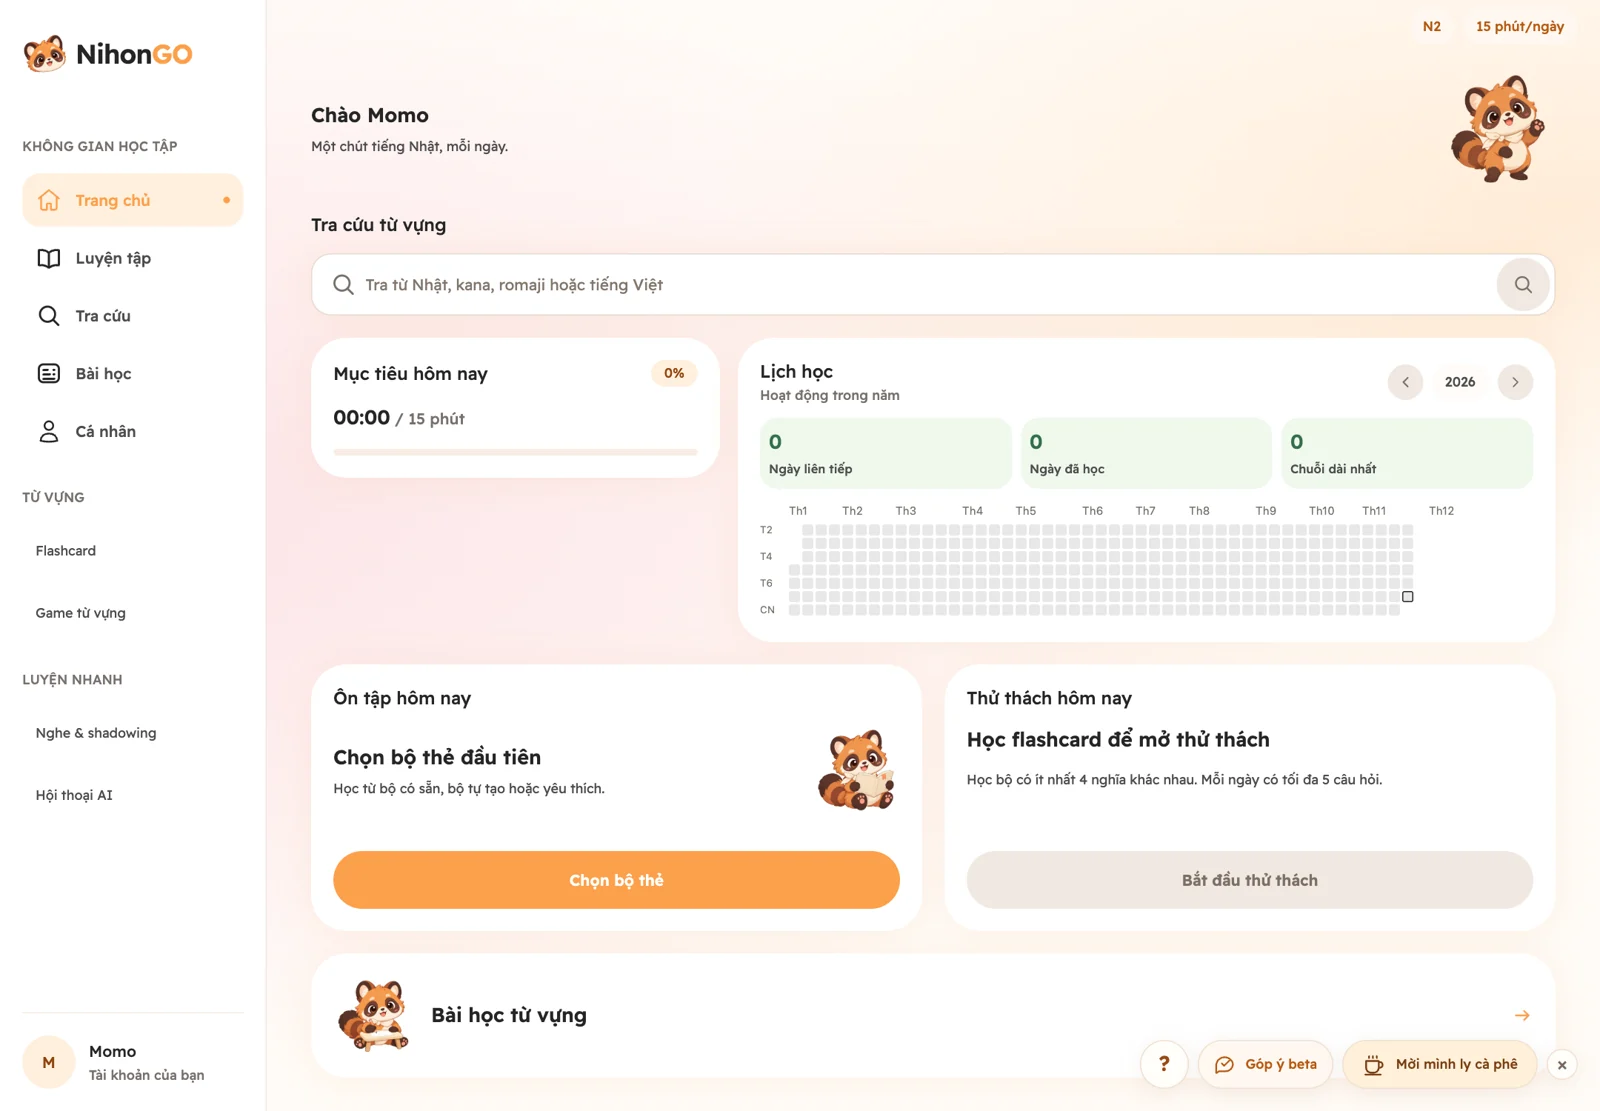
\includegraphics[width=.94\linewidth,height=.365\textheight,keepaspectratio]{figures/mvp/web-home.png}
  \captionof{figure}{Trang chủ và các hoạt động học tập}
  \label{fig:mvp-home}
\end{minipage}
\clearpage
\noindent\begin{minipage}{\linewidth}
  \centering
  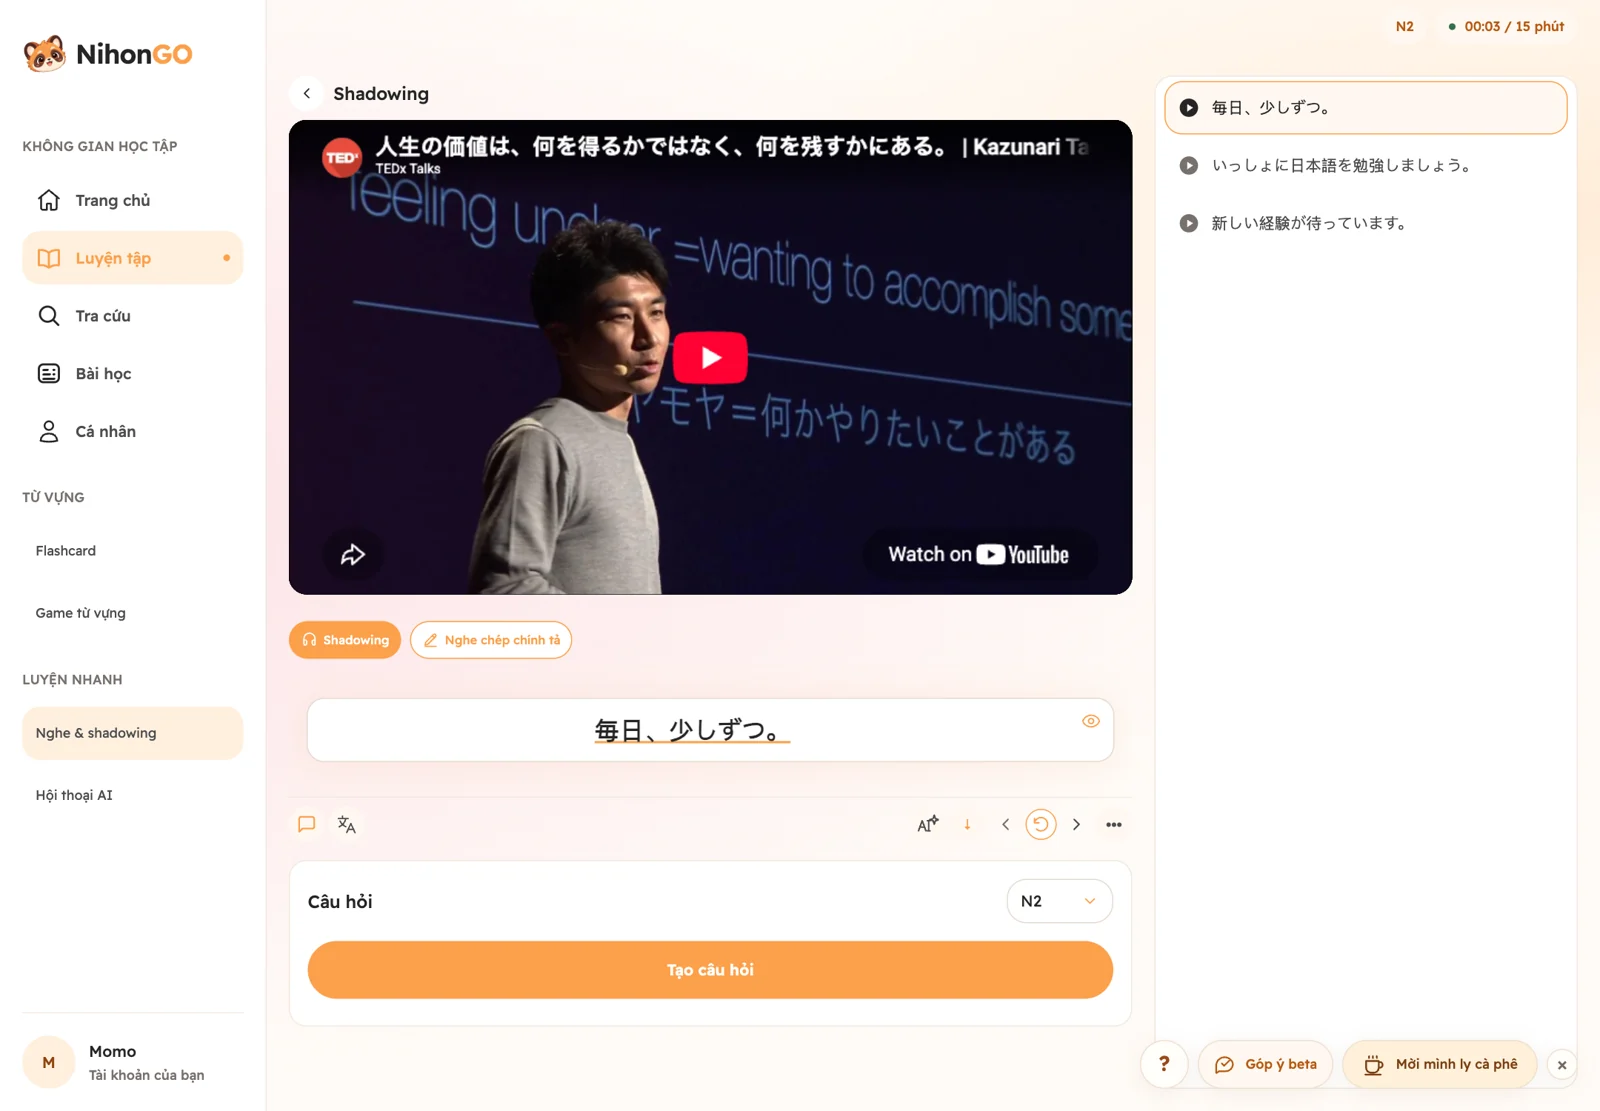
\includegraphics[width=.94\linewidth,height=.365\textheight,keepaspectratio]{figures/mvp/web-shadowing.png}
  \captionof{figure}{Luyện shadowing với video và phụ đề}
  \label{fig:mvp-shadowing}
\end{minipage}

\par\bigskip
\noindent\begin{minipage}{\linewidth}
  \centering
  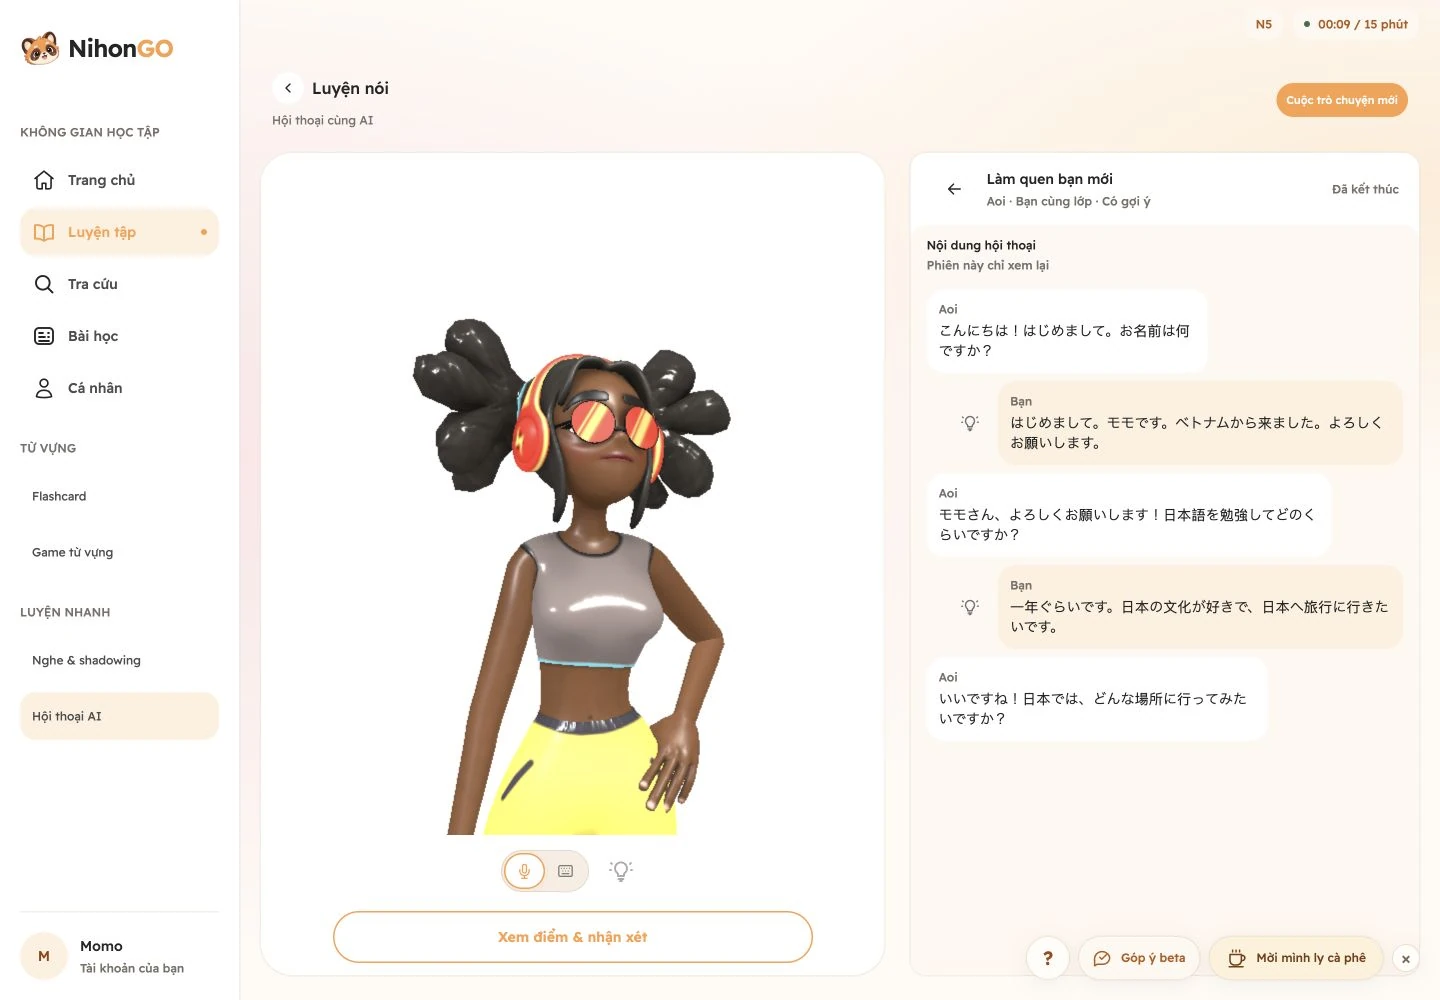
\includegraphics[width=.94\linewidth,height=.365\textheight,keepaspectratio]{figures/mvp/web-speaking-conversation.png}
  \captionof{figure}{Hội thoại theo tình huống với AI}
  \label{fig:mvp-speaking}
\end{minipage}
\clearpage
\noindent\begin{minipage}{\linewidth}
  \centering
  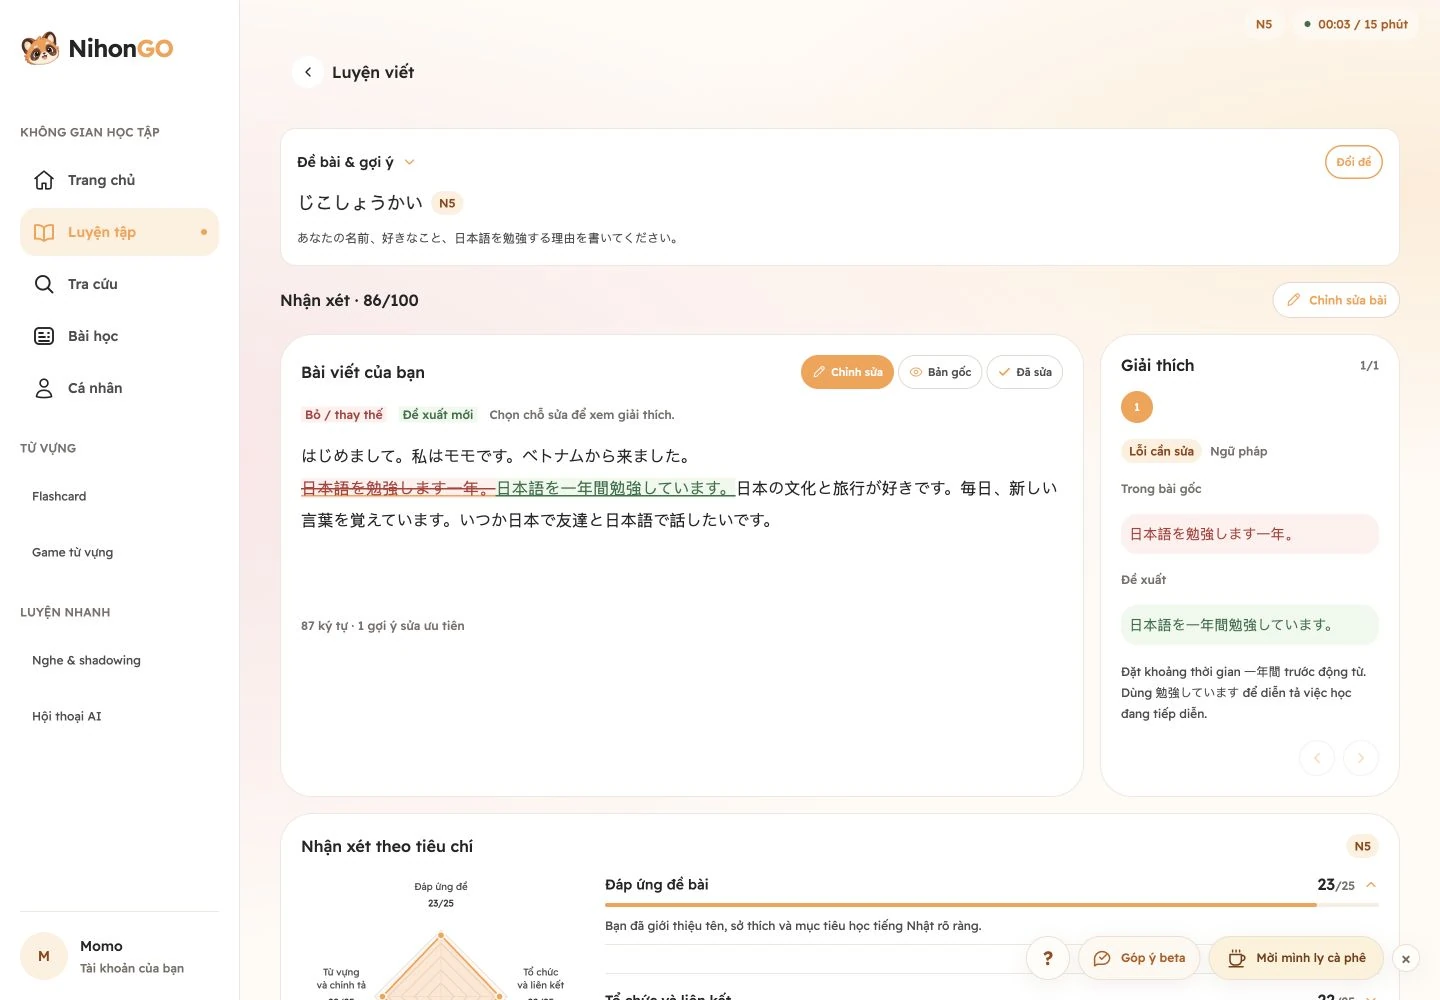
\includegraphics[width=.94\linewidth,height=.365\textheight,keepaspectratio]{figures/mvp/web-writing-feedback.png}
  \captionof{figure}{Nhận xét bài viết và giải thích chỉnh sửa}
  \label{fig:mvp-writing-feedback}
\end{minipage}
\par

\subsection{Case Study}
\section{TESTING AND EVALUATION}
\subsection{Testing Results}
\subsection{User Feedback}
\section{EFFECTIVENESS ANALYSIS}
\section{STARTUP ORIENTATION AND COMMERCIALIZATION}
\subsection{Business Model Canvas}
\subsection{Lean Startup and Design Thinking}
\section{CHAPTER SUMMARY}
   % Chapter 3. Deployment & business models
% =====================================================================
%  CHAPTER 5. CONCLUSION AND RECOMMENDATIONS  (<= 5 pages)
%  Headings only (form).
% =====================================================================
\chapter{Conclusion and Recommendations}

\section{MAIN RESULTS}
\section{INNOVATION VALUE AND APPLICABILITY}
\section{LIMITATIONS}
\section{RECOMMENDATIONS AND PRODUCT ROADMAP}
\subsection{Recommendations}
\subsection{Product Roadmap}
   % Chapter 4. Conclusion & recommendations

% --------------------- References & appendices -----------------------
% Roman numerals continuing the front sequence (References = vi, ...),
% page number bottom right, no header/footer text (QD 675, sec. 1).
\clearpage
\pagenumbering{roman}
\setcounter{page}{\numexpr\FrontLastPage+1\relax}
\pagestyle{front}
\fancypagestyle{plain}{%
  \fancyhf{}\fancyfoot[R]{\thepage}%
  \renewcommand{\headrulewidth}{0pt}\renewcommand{\footrulewidth}{0pt}}

% Tài liệu được nhóm theo ngôn ngữ, xếp theo tác giả/tổ chức.
% Nguồn trực tuyến được tra cứu ngày 23/11/2026.
\phantomsection
\addcontentsline{toc}{chapter}{REFERENCES}
\chapter*{REFERENCES}

\begin{refslist}
  \item[] \hspace*{-0.68cm}\textbf{Vietnamese}
  \bibitem{nihongo-functional2026} Nhóm thực hiện NihonGO (2026),
    \textit{Đặc tả yêu cầu chức năng NihonGO}, tệp
    \nolinkurl{02_FunctionalRequirement.xlsx}, tài liệu nội bộ.
  \bibitem{nihongo-survey2026} Nhóm thực hiện NihonGO (2026),
    \textit{Khảo sát nhu cầu học tiếng Nhật}, dữ liệu khảo sát do nhóm
    cung cấp, 48 phản hồi ghi nhận từ ngày 16/09/2026 đến ngày 17/11/2026,
    tài liệu nội bộ, thông tin liên hệ không công bố.

  \item[] \hspace*{-0.68cm}\textbf{English}
  \bibitem{anki-scheduler} Anki (n.d.),
    \textit{What spaced repetition algorithm does Anki use?},
    \url{https://docs.ankiweb.net/faqs/what-spaced-repetition-algorithm},
    accessed November 23, 2026.
  \bibitem{duolingo-videocall} Duolingo (n.d.),
    \textit{Duolingo's Video Call Offers Realistic Conversation Practice},
    \url{https://blog.duolingo.com/video-call/},
    accessed November 23, 2026.
  \bibitem{gemini-audio} Google (n.d.),
    \textit{Audio understanding}, Gemini API documentation,
    \url{https://aistudio.google.com/docs/audio},
    accessed November 23, 2026.
  \bibitem{hbs-fiveforces} Harvard Business School,
    Institute for Strategy and Competitiveness (n.d.),
    \textit{The Five Forces},
    \url{https://www.isc.hbs.edu/strategy/business-strategy/Pages/the-five-forces.aspx},
    accessed November 23, 2026.
  \bibitem{jpf2024} Japan Foundation (2025, updated April 6, 2026),
    \textit{Survey Summary on Japanese-Language Education Abroad 2024},
    pp.~3, 6--7, 17,
    \url{https://www.jpf.go.jp/e/project/japanese/survey/result/information/dl/result_overview_e_20260406.pdf},
    accessed November 23, 2026.
  \bibitem{mazii-app} Mazii (n.d.),
    \textit{Mazii: Japanese Dictionary}, developer's product description,
    Apple App Store,
    \url{https://apps.apple.com/vn/app/mazii-japanese-dictionary/id933081417},
    accessed November 23, 2026.
  \bibitem{quizlet-flashcards} Quizlet (n.d.),
    \textit{Studying with Flashcards}, Quizlet Help Center,
    \url{https://help.quizlet.com/hc/en-us/articles/360030988091-Studying-with-Flashcards},
    accessed November 23, 2026.
  \bibitem{quizlet-learn} Quizlet (n.d.),
    \textit{Studying with Learn}, Quizlet Help Center,
    \url{https://help.quizlet.com/hc/en-us/articles/360030986971-Studying-with-Learn},
    accessed November 23, 2026.
\end{refslist}
  % References -- numbered [n], grouped by language
% =====================================================================
%  APPENDICES (optional, <= 10 pages). Delete the \input line in
%  main.tex if unused. Appendices are lettered: APPENDIX A, B, ...
% =====================================================================
\appendix

\chapter{Installation and User Guide}
\chapter{Source Code Structure}
    % Appendices (optional)

\end{document}
